\documentclass[12pt]{article} 
%\usepackage{times,helvet}
\usepackage{palatino}
%\usepackage[utf8]{inputenc} %useful to type directly diacritic characters
%\usepackage{ssss}
\usepackage{amsmath,amsbsy,amssymb}
\usepackage{sectsty,hangcaption}
\usepackage{deflist}
\usepackage{fancyhdr}
\usepackage{tabularx}
\usepackage{verbatim}
\usepackage{comment}
\usepackage{moreverb}
\usepackage{float,comment}
\usepackage{graphicx}
\usepackage{longtable}
%\usepackage{portland}
\usepackage{booktabs}

\usepackage[super,comma,sort]{natbib} 
\bibpunct[, ]{(}{)}{;}{a}{,}{,}

%must be last package
%\usepackage{hyperref}
\usepackage[debug=false, colorlinks=true, pdfstartview=FitV, linkcolor=blue, citecolor=blue, urlcolor=blue, pdfpagelabels=true]{hyperref}

\textwidth 6.5in
\textheight 9.5in
%\topmargin -.1in
\topmargin -.75in
\newlength{\boxwidth}
\setlength{\boxwidth}{5.8in}
\oddsidemargin -0in
\evensidemargin -0in
\headheight 0.25in

\lhead{{\sl PFLOTRAN: Governing Equations}}
\chead{\rm - \thepage\ -}
\rhead{\sl DRAFT: \today}
\cfoot{}

\newcommand\flotran{{\sl FloTran}}
\renewcommand{\baselinestretch}{1.0}
\def\EQ#1\EN{\begin{equation}#1\end{equation}}
\def\BA#1\EA{\begin{align}#1\end{align}}
\def\BS#1\ES{\begin{split}#1\end{split}}
%\newcommand{\EQ}{\begin{equation}}
%\newcommand{\EN}{\end{equation}}
\newcommand{\bcr}{\begin{center}}
\newcommand{\ecr}{\end{center}}
\newcommand{\eq}{\ =\ }
\newcommand{\degc}{$^\circ$C}
\renewcommand{\c}{{\rm CO_2}}
\newcommand{\im}{{\rm imb}}
\newcommand{\m}{{\rm mb}}
\newcommand{\ecm}{{\rm ecm}}
\newcommand{\eff}{{\rm eff}}
\newcommand{\eqr}{{\rm le}}
\newcommand{\equ}{{\rm eq}}
\newcommand{\kin}{{\rm kin}}
\newcommand{\rdx}{{\rm rdx}}
\newcommand{\ind}{{\rm id}}
\newcommand{\dep}{{\rm dp}}
\newcommand{\e}{{\rm{e}}}
\newcommand{\erf}{{\rm{erf}}}
\newcommand{\erfc}{{\rm{erfc}}}
\newcommand{\p}{{\partial}}
\newcommand{\A}{{\mathcal A}}
\newcommand{\B}{{\mathcal B}}
\newcommand{\C}{{\mathcal C}}
\newcommand{\D}{{\mathcal D}}
\newcommand{\E}{{\mathcal E}}
\newcommand{\F}{{\mathcal F}}
\newcommand{\G}{{\mathcal G}}
\newcommand{\I}{{\mathcal I}}
\newcommand{\J}{{\mathcal J}}
\newcommand{\M}{{\mathcal M}}
\newcommand{\cO}{{\mathcal O}}
\renewcommand{\P}{{{\mathcal P}}}
\newcommand{\Q}{{\mathcal Q}}
\newcommand{\R}{{{\mathcal R}}}
\renewcommand{\S}{{\mathcal S}}
\newcommand{\T}{{\mathcal T}}
\newcommand{\W}{{\mathcal W}}
\newcommand{\Y}{{\mathcal Y}}
\newcommand{\Z}{{\mathcal Z}}
\newcommand{\rev}{{\rm rev}}
\newcommand{\irr}{{\rm irr}}
\renewcommand{\a}{{\alpha}}
\newcommand{\abar}{{\bar \alpha}}
\renewcommand{\b}{{\beta}}
\renewcommand{\e}{{\epsilon}}
\newcommand{\s}{{\sigma}}
\renewcommand{\t}{{\tau}}
\renewcommand{\sc}{{g}}
\newcommand{\w}{{\rm H_2O}}
\newcommand{\air}{{\rm N_2}}
\newcommand{\pe}{{\rm Pe}}
\newcommand{\da}{{\rm Da}}
\renewcommand{\k}{{\dot R}^0}
\renewcommand{\L}{\widehat{\mathcal L}}
%\renewcommand{\bar}{\overline}
\newcommand{\dsty}{{\displaystyle}}
\newcommand{\diff}{{\mathcal D}}
\newcommand{\surf}{\equiv \!\!\!}
\newcommand{\bnabla}{\boldsymbol{\nabla}}
\newcommand{\ba}{\boldsymbol{a}}

\newcommand{\balpha}{\boldsymbol{\alpha}}
\newcommand{\bbeta}{\boldsymbol{\beta}}
\newcommand{\bgamma}{\boldsymbol{\gamma}}
\renewcommand{\d}{{\delta}}

\newcommand{\bA}{\boldsymbol{A}}
\newcommand{\bB}{\boldsymbol{B}}
\newcommand{\bb}{\boldsymbol{b}}
\newcommand{\bC}{\boldsymbol{C}}
\newcommand{\bc}{\boldsymbol{c}}
\newcommand{\bcolon}{\boldsymbol{:}}
\newcommand{\bdot}{\boldsymbol{\cdot}}
\newcommand{\bD}{\boldsymbol{D}}
\newcommand{\bE}{\boldsymbol{E}}
\newcommand{\bF}{\boldsymbol{F}}
\renewcommand{\bf}{\boldsymbol{f}}
\newcommand{\bG}{\boldsymbol{G}}
\newcommand{\bg}{\boldsymbol{g}}
\newcommand{\bi}{\boldsymbol{i}}
\newcommand{\bI}{\boldsymbol{I}}
\newcommand{\bJ}{\boldsymbol{J}}
\newcommand{\bK}{\boldsymbol{K}}
\newcommand{\bL}{\boldsymbol{L}}
\newcommand{\bM}{\boldsymbol{M}}
\newcommand{\bn}{\boldsymbol{n}}
\newcommand{\bdelta}{\boldsymbol{\delta}}
\newcommand{\bGamma}{\boldsymbol{\Gamma}}
\newcommand{\bomega}{\boldsymbol{\omega}}
\newcommand{\bOmega}{\boldsymbol{\Omega}}
\newcommand{\bPsi}{\boldsymbol{\Psi}}
\newcommand{\bO}{\boldsymbol{O}}
\newcommand{\bnu}{\boldsymbol{\nu}}
\newcommand{\bdS}{\boldsymbol{dS}}
\newcommand{\bP}{\boldsymbol{P}}
\newcommand{\bq}{\boldsymbol{q}}
\newcommand{\br}{\boldsymbol{r}}
\newcommand{\bR}{\boldsymbol{R}}
\newcommand{\bS}{\boldsymbol{S}}
\newcommand{\bU}{\boldsymbol{U}}
\newcommand{\bu}{\boldsymbol{u}}
\newcommand{\bv}{\boldsymbol{v}}
\newcommand{\bw}{\boldsymbol{w}}
\newcommand{\bx}{\boldsymbol{x}}
\newcommand{\by}{\boldsymbol{y}}
\newcommand{\bY}{\boldsymbol{Y}}
\newcommand{\bz}{\boldsymbol{z}}
\newcommand{\bzero}{\boldsymbol{0}}

\newcommand{\arrows}{~\rightleftharpoons~}
\newcommand{\arrowstab}{\!\!\!\rightleftharpoons\!\!\!}
\newcommand{\longline}{\noindent\rule[-0.1in]{\textwidth}{0.01in}}

\def\water{H$_2$O}
\def\calcium{Ca$^{2+}$}
\def\copper{Cu$^{2+}$}
\def\magnesium{Mg$^{2+}$}
\def\sodium{Na$^+$}
\def\potassium{K$^+$}
\def\uranium{UO$_2^{2+}$}
\def\hion{H$^+$}
\def\bicarbonate{HCO$_3^-$}
\def\cotwo{CO$_2$}
\def\chloride{Cl$^-$}
\def\fluoride{F$^-$}
\def\phosphoricacid{HPO$_4^{2-}$}
\def\nitrate{NO$_3^-$}
\def\sulfate{SO$_4^{2-}$}
\def\souotwooh{$>$SOUO$_2$OH}
\def\sohuotwocothree{$>$SOHUO$_2$CO$_3$}
\def\soh{$>$SOH}

%\renewcommand{\thepage}{\roman{page}}
%\renewcommand{\thepage}{\arabic{page}}
%\renewcommand{\theequation}{\arabic{section}.\arabic{subsection}-\arabic{equation}}
%\renewcommand{\theequation}{\arabic{section}-\arabic{equation}}
%\setcounter{page}{1}

\long\def\symbolfootnote[#1]#2{\begingroup%
\def\thefootnote{\fnsymbol{footnote}}\footnote[#1]{#2}\endgroup}

\setlength{\parindent}{0.3125in}
\setlength{\parskip}{2ex plus 0.2ex minus 0.2ex}

\setcounter{secnumdepth}{4}
\setcounter{tocdepth}{4}
\renewcommand{\contentsname}{CONTENTS}

\setlongtables

\pagestyle{fancy}

\thispagestyle{empty}

\author{P.C. Lichtner (LANL)}
\title{Requirements Document for H$_2$O--Supercritical CO$_2$ Two-Phase--Two-Component System}

\begin{document}

\maketitle

\tableofcontents

\section{Scope}

This report provides the governing equations, constitutive relations and numerical considerations for implementing the two-phase--two-component system H$_2$O--CO$_2$ into the SAMRAI parallel adaptive mesh refinement framework. Phases considered are liquid water (H$_2$O) and supercritical carbon dioxide (CO$_2$) designated as $\a = l,\, g$, respectively. Components consist of H$_2$O and CO$_2$ designated alternatively by the subscripts $i$ = $w$ and $c$, respectively. The system considered may be either isothermal, in which case an energy balance equation is not necessary, or nonisothermal increasing the number of degrees of freedom by one.

Even this relatively simple system involves a complex set of nonlinear partial differential equations combined with complex equations of state for material properties and chemical solubility at the relevant temperatures and pressures.

\section{Governing Equations}

\subsection{Mass Conservation Equations}

The governing equations for mass conservation of the $w$ = H$_2$O and $c$ = CO$_2$ components with phases $l$ = liquid H$_2$O and $g$ = supercritical CO$_2$, can be written in the form
\begin{subequations}
\EQ\label{massconv1}
\frac{\p}{\p t} \varphi \big( s_l \rho_l X_w^l + s_g \rho_g X_w^g\big) + \bnabla\cdot\bF_w \eq Q_w,
\EN
and
\EQ\label{massconv2}
\frac{\p}{\p t} \varphi \big( s_l \rho_l X_c^l + s_g \rho_g X_c^g\big) + \bnabla\cdot\bF_c \eq Q_c,
\EN
\end{subequations}
with fluxes
\begin{subequations}
\EQ
\bF_w \eq \bq_l \rho_l X_w^l+ \bq_g \rho_g X_w^g -\varphi s_l \rho_l D_l \bnabla X_w^l-\varphi s_g \rho_g D_g \bnabla X_w^g,
\EN
and 
\EQ
\bF_c \eq \bq_l \rho_l X_c^l+ \bq_g \rho_g X_c^g -\varphi s_l \rho_l D_l \bnabla X_c^l-\varphi s_g \rho_g D_g \bnabla X_c^g,
\EN
\end{subequations}
consisting of contributions from advection and diffusion/dispersion summed over all fluid phases.
In these equations 
\begin{itemize}
\item $\varphi$: porosity [---]
\item $s_l$: the volume fraction in fluid phase liquid water [---]
\item $s_g$: the volume fraction in fluid phase supercritical CO$_2$ [---]
\item $\rho_l$: molar density of liquid water [mol/m$^3$]
\item $\rho_g$: molar density of supercritical CO$_2$ [mol/m$^3$]
\item $D_l$: diffusion/dispersion coefficient for liquid water phase [m$^2$/s]
\item $D_g$: diffusion/dispersion coefficient for supercritical CO$_2$ phase [m$^2$/s]
\item $X_w^l$: mole fraction of the H$_2$O component in fluid phase liquidwater [---] 
\item $X_w^g$: mole fraction of the H$_2$O component in fluid phase supercritical CO$_2$ [---]
\item $X_c^l$: mole fraction of the CO$_2$ component in fluid phase liquid water [---]
\item $X_c^g$: mole fraction of the CO$_2$ component in fluid phase supercritical CO$_2$ [---]
\item $Q_w$: source/sink term for H$_2$O component equation [mol/m$^3$/s]
\item $Q_c$: source/sink term for  CO$_2$ component equation [mol/m$^3$/s]
\item $\bq_l$: Darcy velocity for liquid water phase [m/s]
\item $\bq_g$: Darcy velocity for supercritical CO$_2$ phase [m/s]
\end{itemize}
The equations are over all fluid phases present in a particular control volume. 
The Darcy velocities $\bq_l$ and $\bq_g$ are given by the expressions
\begin{subequations}
\EQ
\bq_l \eq -\frac{kk_l}{\mu_l} \bnabla \Big(P_l - W_l\rho_l g z\Big),
\EN
and
\EQ
\bq_g \eq -\frac{kk_g}{\mu_g} \bnabla \Big(P_g - W_g\rho_g g z\Big),
\EN
\end{subequations}
with:
\begin{itemize}
\item  $P_l$: pressure of fluid phase liquid water [Pa]
\item  $P_g$: pressure of fluid phase supercritical CO$_2$ [Pa]
\item $\mu_l$: viscosity of fluid phase liquid water [Pa s]
\item $\mu_g$: viscosity of fluid phase supercritical CO$_2$ [Pa s]
\item $W_l$: formula weight for the fluid phase liquid water [kg/mol]
\item $W_g$: formula weight for the fluid phase supercritical CO$_2$ [kg/mol]
\item g: acceleration of gravity [m/s$^2$]
\item $z$: elevation [m]
\end{itemize}

The formula weight $W_\a$ for phase $\a$ consisting of a mixture of $N_C$ components is given in general by
\EQ
W_\a \eq \sum_i W_i^{} X_i^\a,
\EN
where $W_i$ [kg/mol] is the formula weight of the $i$th component. 
Substituting, the formula weights into the equations for the Darcy velocities we obtain:
\begin{subequations}
\EQ
\bq_l \eq -\frac{kk_l}{\mu_l} \bnabla \Big(P_l - W_w X_w^l \rho_l g z - W_c X_c^l \rho_l g z \Big),
\EN
and
\EQ
\bq_g \eq -\frac{kk_g}{\mu_g} \bnabla \Big(P_g - W_w X_w^g \rho_l g z - W_c X_c^g \rho_g g z \Big).
\EN
\end{subequations}

We can reformulate Eqns.\eqref{massconv1} and \eqref{massconv2} into an equivalent form which is used in the FLASH method. First, by noting from Eqn.\eqref{sumx} that:
\begin{subequations}
\EQ
X_w^l+X_c^l =1,
\EN
and
\EQ
X_w^g+X_c^g =1,
\EN
\end{subequations}
and summing Eqns.\eqref{massconv1}-\eqref{massconv2} we obtain the pressure equation that we will use in place of Eqn.\eqref{massconv1}:
\EQ\label{massconv3}
\frac{\p}{\p t} \varphi \big( s_l \rho_l + s_g \rho_g \big) + \bnabla\cdot(\bq_l \rho_l + \bq_g \rho_g ) \eq Q_w+Q_c,
\EN

Secondly, we reformulate Eqn.\eqref{massconv2} in terms of the total component mole fraction for CO$_2$, $Z_c$, using the definition in Eqn.\eqref{zi} to obtain the equation we will use in place of Eqn.\eqref{massconv2}:
\EQ\label{mczc}
\frac{\p}{\p t} \varphi \Big( (s_l \rho_l + s_g \rho_g)Z_c \Big) + \bnabla\cdot \bF_c \eq Q_c.
\EN
In this equation the $3$ unknown variables are $(T, \, P,\, Z_c)$. To solve the resulting system of equations it is necessary to express $s_\a$ and $X_i^\a$ as functions of $Z_i$. 

\subsection{Energy Conservation}

The energy conservation equation can be written in the form
\EQ
\sum_\a\left\{\frac{\p}{\p t} \big(\varphi s_\a \rho_\a U_\a\big) + \bnabla\cdot\big(\bq_\a \rho_\a H_\a\big) \right\} + \frac{\p}{\p t} \big(\rho_r C_p T \big) - \bnabla\cdot\big(\kappa\bnabla T\big) \eq Q_e,
\EN
as the sum of contributions from each fluid phase and rock,
with internal energy $U_\a$ and enthalpy $H_\a$ of fluid phase $\a$, and rock heat capacity $C_p$ and thermal conductivity $\kappa$. The quantity $Q_e$ denotes the heat source/sink term. Internal energy and enthalpy are related through the thermodynamic expression
\EQ
H_\a \eq U_\a + \frac{P_\a}{\rho_\a}.
\EN

\section{Numerical Implementation}

\subsection{Finite Volume Discretization: Independent Variables}

In the following the so-called Flash method is used in which a persistent set of independent variables exist regardless of the which phases are present within a control volume and time $t$. This approach is advantageous for use with multilevel solvers to avoid changes in the independent variables on different levels within a patch as could occur in the variable switching approach. Nevertheless, the Flash variable $Z_i$ is piecewise continuous with a change in slope across phase boundaries.
Significant simplifications are possible for a two-phase--two-component system such as characterizes the liquid plus supercritical CO$_2$ system considered here. For this system $N_P=2$ $(l,\,g)$, and $N_C=2$ $(\rm H_2O,\, CO_2)$. Three distinct states exist in the system corresponding to single liquid, single gas and two-phase liquid-gas states. For a nonisothermal system the three independent variables are taken as $P$, $T$, and $Z_\c$, and for an isothermal system $P$ and $Z_\c$.

%\subsection{Finite Volume Discretization}

\subsection{Residual Function}

Using a finite volume discretization approach, the governing flow and transport equations are discretized according to a sum of accumulation, flux and source/sink terms providing the residual function $R_{in}$ for the $i$th component at the $n$th control volume and $\t+1$st time step $\Delta t_{\t+1}$ given by
\BA
R_{in}^{\t+1} \eq & \left[\big(\varphi  Z_i\sum_\a s_\a \rho_\a\big)_n^{\t+1}-(\varphi Z_i\sum_\a s_\a\rho_\a)_n^\t \right] \frac{V_n}{\Delta t_{\t+1}} 
+ \sum_{\a n'} (F_i^\a )_{nn'}^{\t+1} A_{nn'}
- Q_{in}^{\t+1} V_n^{},
\EA
formulated in terms of the primary variables $T,\, P,\, Z_i$ for use with the Flash approach.
In this equation the sum over $n'$ is over all control volumes which are connected to the $n$th control volume with volume $V_n$ and interfacial area $A_{nn'}$. The descritzed form of the flux $(F_{i}^\a)_{nn'}^{\t+1}$ is given by
\EQ
(F_i^\a)_{nn'}^{\t+1} \eq (q_{\a}\rho_{\a}X_{i}^{\a})_{nn'}^{\t+1} -(\varphi s_{\a} \rho_\a D_\a)_{nn'}^{\t+1} \frac{X_{i n'}^{\a, \t+1}-X_{i n}^{\a,\t+1}}{d_{n'}+d_n},
\EN
consisting of contributions from advection and diffusion, where the distances $d_n$, $d_{n'}$ refer to the perpendicular distance from the control volume center to the interface. Special consideration is necessary for quantities evaluated at the interface $n\!-\!n'$ denoted by $(~)_{nn'}$.
In evaluating the residual function the quantities $s_\a$ and $X_i^\a$ are expressed as functions of $Z_i$.

By summing over all components and making use of the constraint condition Eqn.\eqref{sumzi} it is possible to eliminate one residual component equation and replace it with the pressure equation
\BA
R_{n}^{\t+1} \eq &\sum_\a \Big[\big(\varphi s_\a \rho_\a)_n^{\t+1} -(\varphi s_\a \rho_\a)_n^\t \Big] \frac{V_n}{\Delta t_{\t}} + \sum_{\a n'} (F_\a )_{nn'}^{\t+1} A_{nn'}- Q_{n}^{\t+1} V_n^{},
\EA
with
\EQ
(F_\a)_{nn'}^{\t+1} \eq \sum_i (F_i^\a)_{nn'}^{\t+1} \eq (q_{\a}\rho_{\a})_{nn'}^{\t+1},
\EN
where
\EQ
R_n \eq \sum_i R_{in},
\EN
and
\EQ
Q_n \eq \sum_i Q_{in}.
\EN
Note that the sum over the diffusive flux vanishes.

The above formulation applies to both structured and unstructured grids, and cartesian, spherical or cylindrical geometries with appropriately chosen surface areas and volumes.


\begin{comment}

\subsection{Jacobian Matrix}

The Jacobian matrix for an isothermal system has the form
\EQ
\renewcommand{\arraystretch}{2.0} 
\bJ \eq 
\begin{bmatrix}
\dfrac{\p R_P}{\p P} & \dfrac{\p R_P}{\p Z} \\
\dfrac{\p R_Z}{\p P} & \dfrac{\p R_Z}{\p Z}
\end{bmatrix}.
\EN
For a nonisothermal system there is an addition equation for the temperature
\EQ
\renewcommand{\arraystretch}{2.0} 
\bJ \eq 
\begin{bmatrix}
\dfrac{\p R_P}{\p P} & \dfrac{\p R_P}{\p T} & \dfrac{\p R_P}{\p Z} \\
\dfrac{\p R_T}{\p P} & \dfrac{\p R_T}{\p T} & \dfrac{\p R_T}{\p Z} \\
\dfrac{\p R_Z}{\p P} & \dfrac{\p R_Z}{\p T} & \dfrac{\p R_Z}{\p Z}
\end{bmatrix}.
\EN
\end{comment}

\subsection{Isothermal System}

For an isothermal system the governing equations for the two-component system consisting of H$_2$O and CO$_2$ with independent variables pressure $P$ and total CO$_2$ mole fraction $Z_c$, have the following form 
\EQ
\frac{\p}{\p t} M + \bnabla\cdot\bf \eq Q,
\EN
for the pressure equation, and
\EQ
\frac{\p}{\p t} MZ_c + \bnabla\cdot(\bf_l X_c^l + \bf_g X_c^g + \bf_{Dc}^l + \bf_{Dc}^g) \eq Q_{c},
\EN
for the total $c$ = CO$_2$ mole fraction $Z_c$. In these equations
\EQ
M \eq \varphi (s_l^{} \rho_l^{} + s_g^{} \rho_g^{}),
\EN
and
\EQ
\bf \eq \bf_l^{} + \bf_g^{},
\EN
with
\EQ
\bf_l^{} \eq \bq_l^{} \rho_l^{},
\EN
and
\EQ
\bf_g^{} \eq \bq_l^{} \rho_g^{}.
\EN
The liquid and gas diffusive fluxes $\bf_{Dc}^l$ and $\bf_{Dc}^g$ have the form
\EQ
\bf_{Dc}^l \eq -\varphi \tau s_l^{} \rho_l^{} D_l \bnabla X_c^l,
\EN
and
\EQ
\bf_{Dc}^g \eq -\phi\tau s_g D_{g}^0 \left(\dfrac{T}{T_K}\right)^\theta \dfrac{P_0}{P_g}\nabla X_c^g,
\EN
with $T_K = 273.15$ K, $P_0$ represents a reference pressure, $\tau$ is tortuosity, $\theta$ is a parameter typically with the value 1.8, and $D_{g}^0$ denotes the diffusion coefficient at reference conditions with the typical value $2.13 \times 10^{-5}$ m$^2$/s. 

The source/sink terms are given by
\EQ
Q \eq \Big[W_\w^{-1} q_{l}^{M} + W_\c^{-1} q_{g}^{M}\Big] \delta(\br-\br_W),
\EN
and
\EQ
Q_c \eq \Big[W_\w^{-1} q_l^M X_c^l + W_\c^{-1} q_g^M X_c^g\Big]\delta(\br-\br_W),
\EN
where $q_{\a}^M$ denotes the mass rate [kg/s] for injection and withdrawal at the well located at $\br_W$. A positive value represents injection and a negative value withdrawal.

The residual function for the pressure equation is calculated for a 3D nine-point orthogonal stencil using the notation for the $(i,\,j,\,k)$th-grid block
\BA
R_{Pn} \eq \frac{\Delta_t M_n}{\Delta t}V_n &+ f_{i+1/2} A_{i+1/2}-f_{i-1/2} A_{i-1/2} \nonumber\\
&+ f_{j+1/2} A_{j+1/2}-f_{j-1/2} A_{j-1/2}\nonumber\\
&+ f_{k+1/2} A_{k+1/2}-f_{k-1/2} A_{k-1/2}\nonumber\\
& - \Big[W_\w^{-1} q_{l}^{M} + W_\c^{-1} q_{g}^{M}\Big] V_n \delta_{nW},
\EA
with
\EQ
\Delta_t M_n \eq M_n^{\tau+1}-M_n^\tau,
\EN
and
with $n\!=\!i\!+\!(j\!-\!1)N_x \!+\! (k\!-\!1)N_x N_y$, where number of grid blocks in the $x$, $y$ and $z$ directions are equal to $N_x$, $N_y$ and $N_z$ with volume $V_n$ and interfacial area $A_{nn'}$. A fully implicit formulation is used with the flux terms evaluated at the new time level $\tau+1$.


The residual function for component $c$ = CO$_2$ is given by
\BA
R_{Z_c n} \eq \frac{\Delta_t (MZ_c)_n}{\Delta t}V_n &+ (f_l X_c^l + f_g X_c^g + f_{Dc}^l+f_{Dc}^g)_{i+1/2} A_{i+1/2}\nonumber\\
&-(f_l X_c^l + f_g X_c^g + f_{Dc}^l+f_{Dc}^g)_{i-1/2} A_{i-1/2}\nonumber\\
&+(f_l X_c^l + f_g X_c^g + f_{Dc}^l+f_{Dc}^g)_{j+1/2} A_{j+1/2}\nonumber\\
&-(f_l X_c^l + f_g X_c^g + f_{Dc}^l+f_{Dc}^g)_{j-1/2} A_{j-1/2}\nonumber\\
&+(f_l X_c^l + f_g X_c^g + f_{Dc}^l+f_{Dc}^g)_{k+1/2} A_{k+1/2}\nonumber\\
&-(f_l X_c^l + f_g X_c^g + f_{Dc}^l+f_{Dc}^g)_{k-1/2} A_{k-1/2}\nonumber\\
&-\Big[W_\w^{-1} q_{l}^{M}X_c^l + W_\c^{-1} q_{g}^{M}X_c^g\Big] V_n \delta_{nW},
\EA
with flux terms evaluated at the new time step.

\subsubsection{Accumulation Terms}

\paragraph{Single Liquid Phase.} The independent variables are $P\!=\!P_l$ and $Z_c\!=\!X_c^l$ with $s_g\!=\!0, \ s_l\!=\!1$.
~

\noindent {\sl Total accumulation (pressure equation):}
\EQ
M_{P} \eq \varphi \rho_l,
\EN
\BA
\delta M_{P} &\eq \varphi \delta\rho_l,\nonumber\\
&\eq \varphi\big(\rho_{lP}^{}\delta P+\rho_{lZ}^{} \d Z_c^{}\big),
\EA
where the notation
\EQ
\rho_{lP}^{} \eq \left(\frac{\p\rho_l}{\p P}\right)_{Z_c},
\EN
etc. is used.

\noindent {\sl Component $Z_\c$:}
\EQ
M_{Z_c} \eq \varphi \rho_l Z_c^{},
\EN
\BA
\delta M_{Z_c} &\eq \varphi (\delta\rho_l^{} Z_c^{}+\rho_l^{}\delta Z_c^{}),\nonumber\\
&\eq \varphi\big(\rho_{lP}^{}Z_c^{}\delta P + (\rho_l^{}+\rho_{lZ}^{})\delta Z_c^{}\big).
\EA

\paragraph{Single Gas Phase.} The independent variables are $P\!=\!P_g$ and $Z_c\!=\!X_c^g$ with $s_g\!=\!1, \ s_l\!=\!0$.
~

\noindent {\sl Total accumulation:}
\EQ
M_{P} \eq \varphi \rho_g,
\EN
\BA
\delta M_{P} &\eq \varphi \delta\rho_g,\nonumber\\
&\eq \varphi\rho_{gP}^{}\delta P.
\EA

\noindent {\sl Component $Z_\c$:}
\EQ
M_{Z_c} \eq \varphi \rho_g Z_c^{},
\EN
\BA
\delta M_{Z_c} &\eq \varphi (\delta\rho_l Z_c^{} +\rho_g^{}\delta Z_c^{}),\nonumber\\
&\eq \varphi\big(\rho_{gP}^{}Z_c^{}\delta P + (\rho_g^{}+\rho_{gZ_c}^{})\delta Z_c^{}\big).
\EA

\paragraph{Two-Phase.} The independent variables are $P\!=\!P_g$ and $Z_c$ with $s_g+s_l\!=\!1$, and with liquid pressure related to gas pressure and the total mole fraction through capillary pressure by 
\EQ
P_l(P_g,\,Z_c) \eq P_g - P_c\big(s_g(P_g,\,Z_c)\big),
\EN
where $P_c$ refers to capillary pressure (see Eqn.\eqref{pc}), and the functional dependence of the gas saturation $s_g$ is obtained from the relation
\EQ
s_g (P_g,\,Z_c) \eq \frac{\rho_l^{} (Z_c^{}-X_c^l)}{\rho_l^{} (Z_c^{} - X_c^l) - \rho_g^{} (Z_c^{}-X_c^g)},
\EN
according to Eqn.\eqref{sg}. It should be noted that the composition variables $X_i^\a$ are invariant depending only on temperature and pressure and not $Z_c$.
Changes in density and saturation in terms of the independent variables are equal to
\begin{subequations}
\BA
\d\rho_l^{} &\eq \rho_{lP}^{}(\d P-\d P_c^{}) + \rho_{lZ_c}^{}\d Z_c^{},\nonumber\\
&\eq \rho_{lP}^{}(1-P_{cs_g}^{}s_{gP}^{})\d P + (\rho_{lZ_c}^{}-P_{cs_g}^{} s_{gZ_c}^{})\d Z_c^{},\\
\d\rho_g^{} &\eq \rho_{gP}^{}\d P + \rho_{gZ_c}^{}\d Z_c^{},\\
%\text{and}&\\
\d s_g &\eq s_{gP}^{}\d P + s_{gZ_c}^{}\d Z_c^{}.
\EA
\end{subequations}

\noindent {\sl Total accumulation:}
\EQ
M_{P} \eq \varphi (s_l\rho_l+s_g\rho_g),
\EN
\BA
\delta M_{P} &\eq \varphi (s_l\delta\rho_l+s_g\delta\rho_g )+\varphi (\rho_g-\rho_l)\delta s_g,\nonumber\\
&\eq \varphi\big(s_l^{}\rho_{lP}^{}+s_g\rho_{gP}^{} + (\rho_g^{}-\rho_l^{}) s_{gP}^{} \big) \delta P + \varphi(\rho_g^{}-\rho_l^{}) s_{gZ_c}^{} \delta Z_c.
\EA

\noindent {\sl Component $Z_\c$:}
\EQ
M_{Z_c} \eq \varphi Z_c^{}(s_l\rho_l+s_g\rho_g),
\EN
\BA
\delta M_{Z_c} &\eq \varphi Z_c^{} (s_l^{}\delta\rho_l^{} + s_g^{}\delta\rho_g^{})
+ \varphi Z_c^{} (\rho_g^{}-\rho_l^{}) \delta s_g^{} 
+ \varphi (s_l^{}\rho_l^{}+s_g^{}\rho_g^{})\delta Z_c^{},\nonumber\\
&\eq \varphi Z_c^{} \big(s_l^{}\rho_{lP}^{}+s_g^{}\rho_{gP}^{}
+ (\rho_g^{}-\rho_l^{}) s_{gP}^{}\big) \delta P \nonumber\\
&\qquad + \varphi \big( Z_c^{}(\rho_g^{}-\rho_l^{}) s_{gZ_c}^{} 
+ s_l^{}\rho_l^{}+s_g^{}\rho_g^{}\big) \delta Z_c^{}.
\EA

\subsubsection{Flux Terms}

The total flux in the $x,\,y,\,z$-directions for the pressure equation is given by 
\begin{subequations}
\EQ
\Delta_x f_x \eq \Delta_x \left(f_{lx}+f_{gx}\right) \eq \left(\rho_l q_l+\rho_g q_g \right)_{i+1/2}^{\t+1} A_{i+1/2}-\left( \rho_l q_l+\rho_g q_g \right)_{i-1/2}^{\t+1}A_{i-1/2},
\EN
\EQ
\Delta_y f_y \eq \Delta_y \left(f_{ly}+f_{gy}\right) \eq \left(\rho_l q_l+\rho_g q_g \right)_{j+1/2}^{\t+1} A_{j+1/2} -\left(\rho_l q_l+\rho_g q_g \right)_{j-1/2}^{\t+1} A_{j-1/2},
\EN
and
\EQ
\Delta_z f_z \eq \Delta_z \left(f_{lz}+f_{gz}\right) \eq \left(\rho_l q_l+\rho_g q_g \right)_{k+1/2}^{n+1} A_{k+1/2} -\left(\rho_l q_l+\rho_g q_g \right)_{k-1/2}^{\t+1} A_{k-1/2}.
\EN
\end{subequations}

Similarly, for the $Z_\c$-equation with $c$ = $\c$ one has
\begin{subequations}
\BA
\Delta_x f_{cx} \eq \Delta_x \left(f_{lx}^{}X_c^l+f_{gx}^{} X_c^g\right) \eq &\left(\rho_l q_l X_c^l+\rho_g q_g X_c^g\right)_{i+1/2}^{\t+1} A_{i+1/2}\nonumber\\
&-\left(\rho_l q_l X_c^l+\rho_g q_g X_c^g\right)_{i-1/2}^{\t+1} A_{i-1/2}\nonumber\\
&+ (f_{cD}^l + f_{cD}^g)_{i+1/2}^{\t+1} A_{i+1/2}\nonumber\\
&-(f_{cD}^l + f_{cD}^g)_{i-1/2}^{\t+1} A_{i-1/2},
\EA
\BA
\Delta_y f_{cy} \eq \Delta_y \left(f_{ly}^{}X_c^l+f_{gy}^{} X_c^g\right) \eq &\left(\rho_l q_l X_c^l+\rho_g q_g X_c^g \right)_{j+1/2}^{\t+1} A_{j+1/2} \nonumber\\
&- \left(\rho_l q_l X_c^l+\rho_g q_g X_c^g \right)_{j-1/2}^{\t+1} A_{j-1/2}\nonumber\\
&+(f_{cD}^l + f_{cD}^g)_{j+1/2}^{\t+1} A_{j+1/2}\nonumber\\
&-(f_{cD}^l + f_{cD}^g)_{j-1/2}^{\t+1} A_{j-1/2},
\EA
and
\BA
\Delta_z f_{cz} \eq \Delta_z \left(f_{lz}^{}X_c^l+f_{gz}^{} X_c^g\right) \eq &\left(\rho_l q_l X_c^l+\rho_g q_g X_c^g \right)_{k+1/2}^{\t+1} A_{k+1/2} \nonumber\\
&- \left(\rho_l q_l X_c^l+\rho_g q_g X_c^g \right)_{k-1/2}^{\t+1} A_{k-1/2}\nonumber\\
&+(f_{cD}^l + f_{cD}^g)_{k+1/2}^{\t+1} A_{k+1/2}\nonumber\\
&-(f_{cD}^l + f_{cD}^g)_{k-1/2}^{\t+1} A_{k-1/2}.
\EA
\end{subequations}

\begin{table}[h]\centering
\caption{Interface weighting scheme.}\label{tnn}
\label{twt}

\vspace{3mm}

\begin{tabular}{lcr}
\toprule
Property & Symbol & \multicolumn{1}{r}{Interface Average}\\
\midrule
Density & $\rho_\a$ & Arithmetic Average\\
%$H_\a$ & Arithmetic Average\\
Permeability & $k$ & Harmonic Average\\
Mobility & $\lambda_\a$ & Upstream Weighting\\
Mole Fraction & $X_i^{\a}$ & Upstream Weighting\\
\bottomrule
\end{tabular}
\end{table}

The liquid flux at the $i\!-\!1/2$ face can be expressed as
\EQ
f_{x,i-1/2}^l \eq \frac{(k \lambda_l \rho_l)_{i-1/2}}{d_i+d_{i-1}} \Phi_{li} A_{i-1/2},
\EN
where the potential difference $\Phi_{li}$ between grid blocks separated by a vertical distance $\Delta z_i$ is given by
\EQ
\Phi_{li}^{} \eq \Delta P_i^l - \gamma_{l,i-1/2}^{} \Delta z_i^{},
\EN
where
\EQ
\Delta P_i^l \eq P_{i}^l -P_{i-1}^l.
\EN
The mobility $\lambda_l$ is given by
\EQ
\lambda_l \eq \frac{k_{l}}{\mu_l},
\EN
where $k_l$ denotes the relative permeability, in general a nonlinear function of saturation, and the quantity $\gamma_l$ is defined by
\EQ
\gamma_l^{} \eq W_l^{} \rho_l g,
\EN
with $g$ the acceleration of gravity.

Interface properties are calculated according to the schemes listed in Table~\ref{tnn}. The permeability is calculated as the harmonic average of $k_{i-1}$ and $k_i$, the density is taken as the arithmetic average, and the mobility is averaged based on a weighting factor applied to the upstream block. Thus
\BA
k_{i-1/2} \eq \frac{(d_i+d_{i-1})k_ik_{i-1}}{d_i k_{i-1}+d_{i-1} k_i},\\
\EA
The fluid density at the interface is given by
\EQ
\rho_{l,i-1/2} \eq \frac{d_i\rho_{l,i}+d_{i-1}\rho_{l,i-1}}{d_i+d_{i-1}},
\EN
with the derivative
\BA
\d\rho_{l,i-1/2} &\eq \frac{d_i\d\rho_{l,i}+d_{i-1}\d\rho_{l,i-1}}{d_i+d_{i-1}},\\
&\eq \frac{d_i(\rho_{l,P_i}^{})\d P_i+d_{i-1}(\rho_{l,P_{i-1}}^{}) \d P_{i-1}}{d_i+d_{i-1}}
\EA
Mobility is upstream weighted
\EQ
\lambda_{l,i-1/2} \eq \lambda_{lu},
\EN
where the subscript $u$ refers to the upstream grid block. 
Upstream weighting is also used for the $\c$ mole fraction $X_\c^{l,\,g}$.
\EQ
(X_\c^{l,\,g})_{i-1/2}^{} \eq (X_\c^{l,\,g})_{u}^{}.
\EN

Substituting the quantities as defined above, the flux at the
interface is given by
\EQ\label{liqflx}
f_{x,i-1/2}^l \eq \T_{x,i-1/2}^{} \, \rho_{l,i-1/2}^{} \, \lambda_{l,i-1/2}^{} \, \Phi_{li}^{},
\EN
where the transmissibility $\T_{x,i-1/2}^{}$ is defined by
\EQ
\T_{x,i-1/2} \eq \frac{k_i k_{i-1}}{d_i k_{i-1} + d_{i-1} k_i} A_{i-1/2}.
\EN
Note that for $i \!=\! 1$, the transmissibility $\T_{x,i-1/2}^{}$ is set to zero, as it is at $n_x\!+\!1$, the outermost interface. This in essence sets the condition of zero flux at the boundary of the system. If
the permeability is constant with time, $\T_{x,i-1/2}^{}$ remains unchanged. 

Similarly, the gas flux can be written analogously as:
\EQ\label{qxg}
f_{x,i-1/2}^g \eq \T_{x,i-1/2}^{} \, \rho_{g,i-1/2}^{} \, \lambda_{g,i-1/2}^{} \, \Phi_{gi}^{},
\EN
where
\EQ
\Phi_{gi} \eq \Delta P_i^g - \gamma_{g,i-1/2} \Delta z_i,
\EN
with
\EQ
\Delta P_i^g \eq P_{i}^g - P_{i-1}^g.
\EN
Fluxes in $y$- and $z$-directions have similar forms. 

\paragraph{Single Liquid Phase}
~

The change in liquid flux is given by
\EQ\begin{split}\label{delf}
\delta f_{l,i-1/2} &\eq \T_{i-1/2}^{} \, \delta(\rho_{l,i-1/2}^{} \, \lambda_{l,i-1/2}^{} \, \Phi_{li}^{}),\\
&\eq \T_{i-1/2}^{} \, (\delta\rho_{l,i-1/2}^{} \, \lambda_{l,i-1/2}^{} \, \Phi_{li}^{}+ \rho_{l,i-1/2}^{} \, \delta\lambda_{l,i-1/2}^{} \, \Phi_{li}^{} + \rho_{l,i-1/2}^{} \, \lambda_{l,i-1/2}^{} \, \delta\Phi_{li}^{}),\\
& \eq \T_{i-1/2} \left[\Phi_{li} \, \lambda_{l,i-1/2} \, \delta \rho_{l,i-1/2} + \Phi_{li} \, \rho_{l,i-1/2} \, \delta \lambda_{l,i-1/2} \right.\\
& \left. \qquad + \rho_{l,i-1/2} \, \lambda_{l,i-1/2} \, (\delta \Delta P_{i}^l - \Delta z_i \delta \gamma_{l,i-1/2})\right].
%-\rho_{l,i-1/2} \, \lambda_{l,i-1/2} \, \delta \Delta P_{ci} 
%+ 2\alpha_{li} \, \delta \rho_{l,i-1/2}
\end{split}
\EN
The variations $\delta \lambda_{l,i-1/2}$, $\delta \rho_{l,i-1/2}$ and $\delta \gamma_{l,i-1/2}$ can expressed in terms of the independent variables $P$ and $Z_c$. It follows that
\begin{align}
\delta \lambda_l &= \frac{d k_l}{ds_g}\frac{ds_g}{dZ_c} \delta Z_c.
%\Delta P_{c,i} &= P_{c,i} - P_{c,{i-1}},\\
%\delta P_c &= \frac{dP_c}{ds_g} \delta s_g,\\
%\alpha_{li} &= \frac{\lambda_{l,i-1/2}}{2} \left(\Phi_{li} - \rho_{l,i-1/2} W_l g \Delta z_i \right).
\end{align}
The change in $c=\c$ flux in the liquid phase can be written in terms of the pressure equation flux and a diffusion term
\EQ
\delta \left(f_l X_c^l + f_D^l\right)_{i-1/2} \eq X_{cu}^l \delta f_{l,i-1/2} + f_{l,i-1/2} \delta X_{c,i-1/2}^l + \delta (f_{cD}^l)_{i-1/2}.
\EN
where
\EQ
(f_{cD}^l)_{i-1/2} \eq -\frac{(\varphi s_l \rho_l D_l)_{i-1/2}}{d_i+d_{i-1}} \big(X_{\c,i}^l-X_{\c,i-1}^l\big).
\EN
Upstream weighting is used for the $\c$ mole fraction $X_\c^l$. The derivative of the diffusive flux is given by
\BA
\delta(f_{cD}^l)_{i-1/2} &\eq -\frac{(\varphi s_l \rho_l D_l)_{i-1/2}}{d_i+d_{i-1}} \delta\big(X_{\c,i}^l-X_{\c,i-1}^l\big) \nonumber\\
&\qquad-\frac{\delta(\varphi s_l \rho_l D_l)_{i-1/2}}{d_i+d_{i-1}} \big(X_{\c,i}^l-X_{\c,i-1}^l\big).
\EA


The derivative of the mole fraction $X_c^\a$ depends on the state of the system
\EQ
\delta X_c^\a \eq \left\{
\renewcommand{\arraystretch}{1.35}
\begin{array}{llc}
0, & \text{two-phase:} & X_\c^{l,\rm eq} < Z_c^{} < X_c^{g,\rm eq}\\
\delta Z_c^{}, & \text{single phase:} & Z_c^{} \leq X_\c^{l,\rm eq} \ \text{or} \ X_\c^{g,\rm eq} \leq Z_c^{}
\end{array}
\right..
\EN

\paragraph{Single Gas Phase}
~

The gas phase flux for advection is similar to the liquid phase. The diffusive flux has the form
\EQ
f_{cD}^g \eq -\phi\tau D_{va}^0 \left(\dfrac{T}{T_K}\right)^\theta \dfrac{P_0}{P_g} s_g\nabla X_c^g,
\EN
with $T_K = 273.15~^\circ$K, $P_0$ represents a reference pressure, $\tau$ is tortuosity, and $\theta$ is a parameter, typically with the value 1.8. 

\paragraph{Two-Phase}
~

\subsection{Source/Sink}

The source/sink terms are given by
\EQ
Q_n \eq \Big[W_\w^{-1} q_{l}^{M} + W_\c^{-1} q_{g}^{M}\Big] \delta_{nW},
\EN
and
\EQ
Q_{cn} \eq \Big[W_\w^{-1} q_l^M X_c^l + W_\c^{-1} q_g^M X_c^g\Big] \delta_{nW}.
\EN

\BA
q_\a^M>0, \ \ \ \d Q_n = 0, \d Q_{cn}=0,\\
q_\a^M<0, \ \ \ \d Q_n = \cdots, \d Q_{cn}=\cdots,
\EA

\section{Example Problem}

An example problem using PFLOTRAN is presented to provide a benchmark problem for comparison with SAMRAI. In this problem supercritical CO$_2$ is injected at a rate of 1 kg/s for 10 years at the center of a domain of size 500 m $\!\times\!$ 500 m $\!\times\!$ 100 m in a grid cell measuring 10 m $\!\times\!$ 10 m $\!\times\!$ 2 m. A coarse grid is used with size 25 $\times$ 25 $\times$ 50. The ambient temperature is taken as 50\degc\ with a pressure of 200 bars.

Results are shown in Figures~\ref{f10y} and \ref{f250y} for times of 10 and 250 years, respectively, for saturation (left) and dissolved CO$_2$ (right). Fingering of dissolved CO$_2$ occurs in the H$_2$O phase as evident in Figure~\ref{f250y}.

Shown in Figure~\ref{fmass} is the total moles of CO$_2$ in the H$_2$O (blue curve) and supercritical CO$_2$ (red curve) phases. The peak in CO$_2$ in the supercritical CO$_2$ phase occurs at 10 years when injection is halted. With increasing time the CO$_2$ in the H$_2O$ increases with time and the supercritical CO$_2$ phase dissipates.

Finally, in Figure~\ref{fzco2} the quantities $Z_\c$, $s_g$, $X_\c^l$ and $X_\c^g$ are plotted at the injection well as a function of time. Note the discontinuity in the slope of these quantities as supercritical CO$_2$ is formed at approximately 0.0004 years indicated by the vertical line in the gas saturation $s_g$. A sharp drop in these quantities is observed at 10 years when injection is halted. The relatively flat top in the curves for $Z_\c$ and $s_g$ which appears just before injection is stopped at 10 years is caused by reaching the residual saturation with a value of 0.1.

\begin{figure}[h]
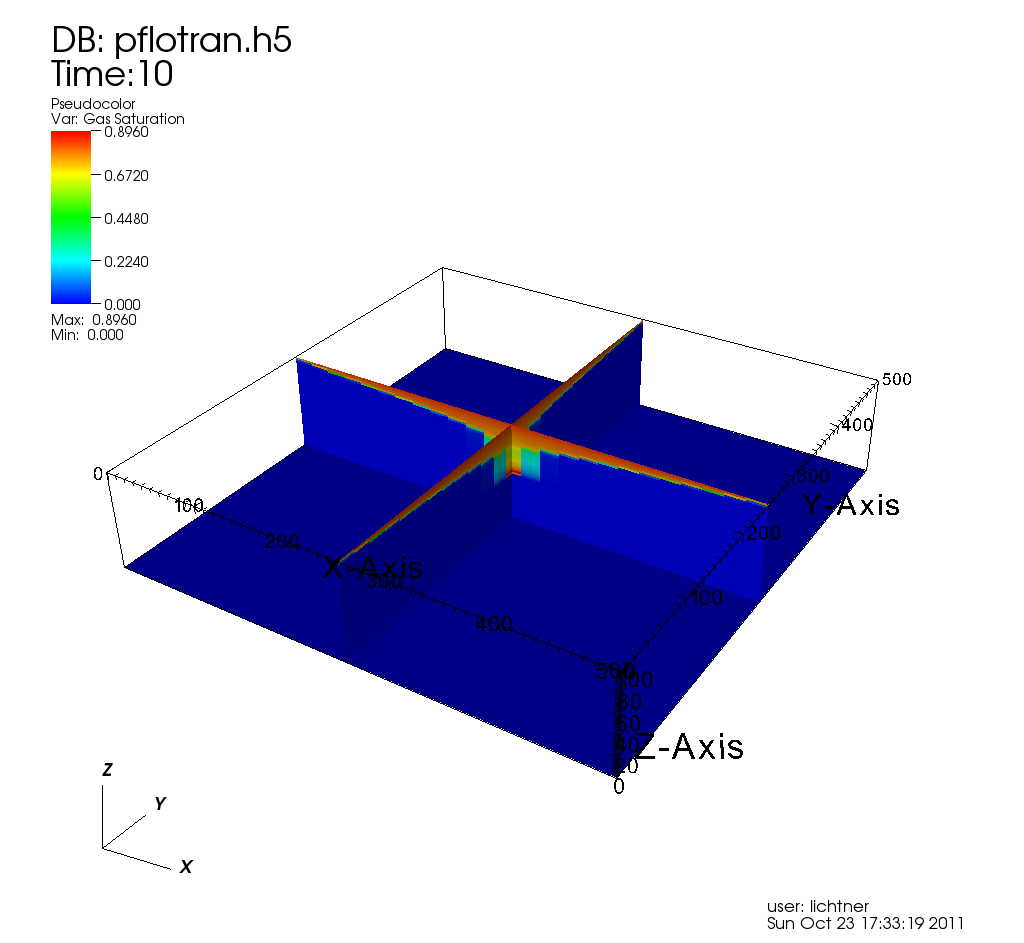
\includegraphics[scale=0.25]{./figs/sg-10y.png}
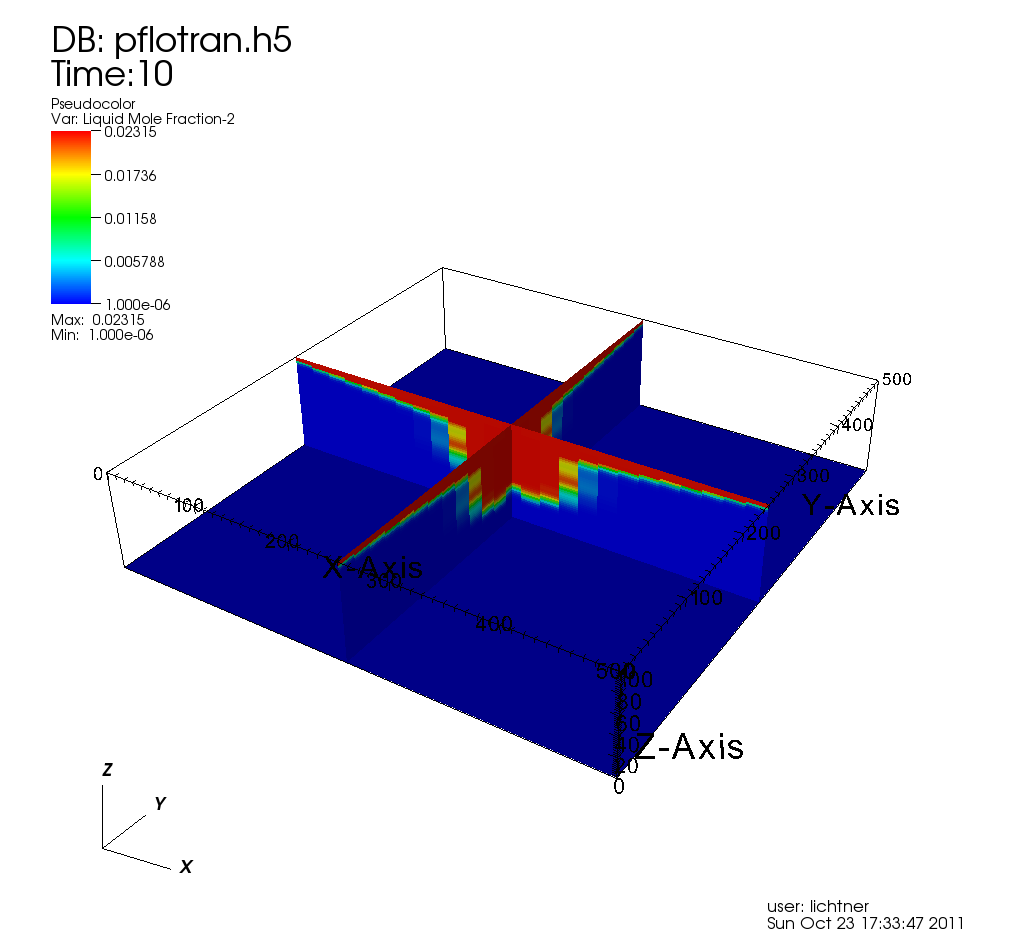
\includegraphics[scale=0.25]{./figs/xlco2-10y.png}
\caption{Saturation of supercritical CO$_2$ (left) and mole fraction of dissolved CO$_2$ (right) at an elapsed time of 10 years when injection is halted.}\label{f10y}
\end{figure}

\begin{figure}
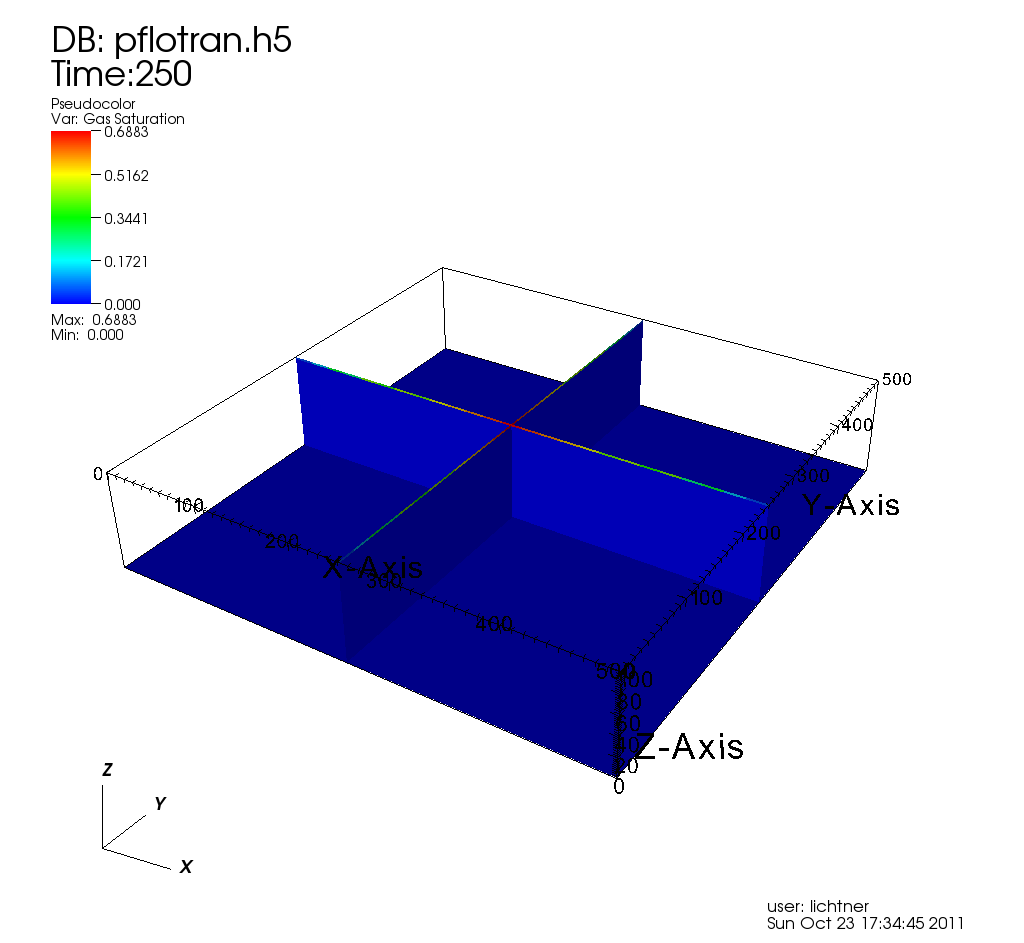
\includegraphics[scale=0.25]{./figs/sg-250y.png}
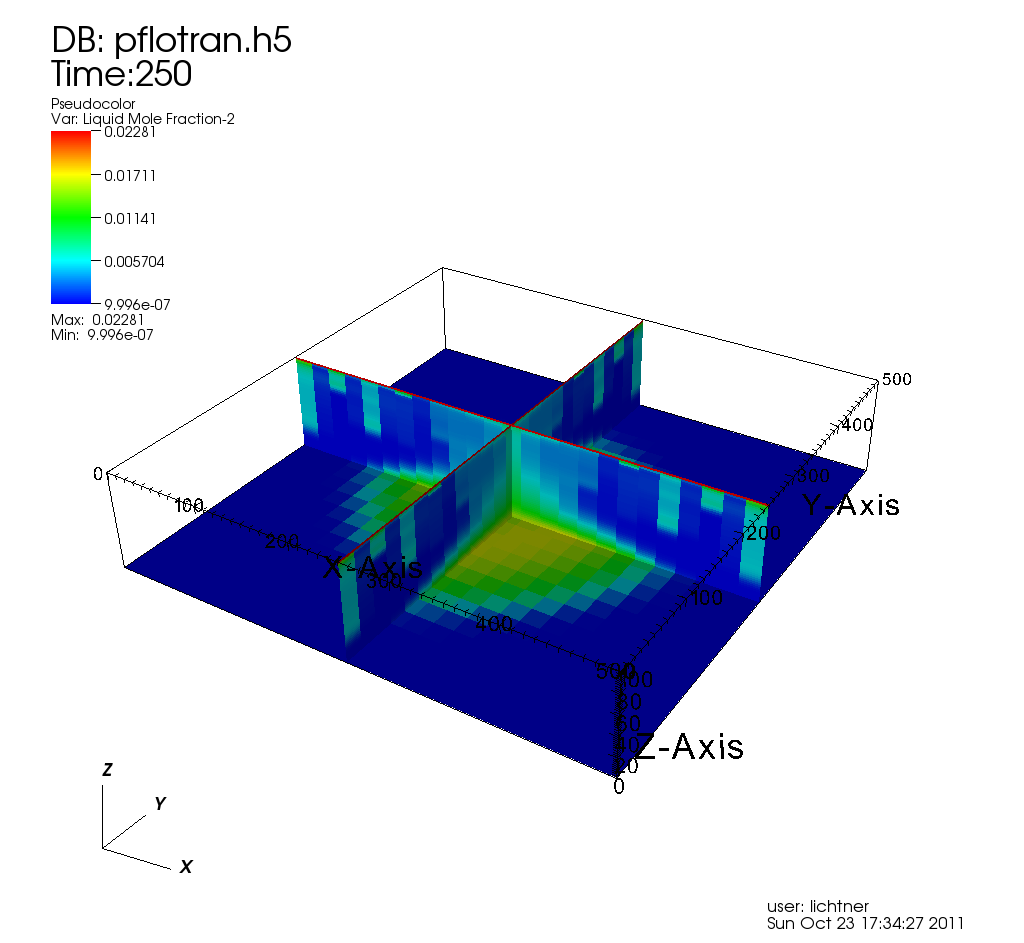
\includegraphics[scale=0.25]{./figs/xlco2-250y.png}
\caption{Saturation of supercritical CO$_2$ (left) and mole fraction of dissolved CO$_2$ (right) at an elapsed time of 250 years.}\label{f250y}
\end{figure}

\begin{figure}\centering
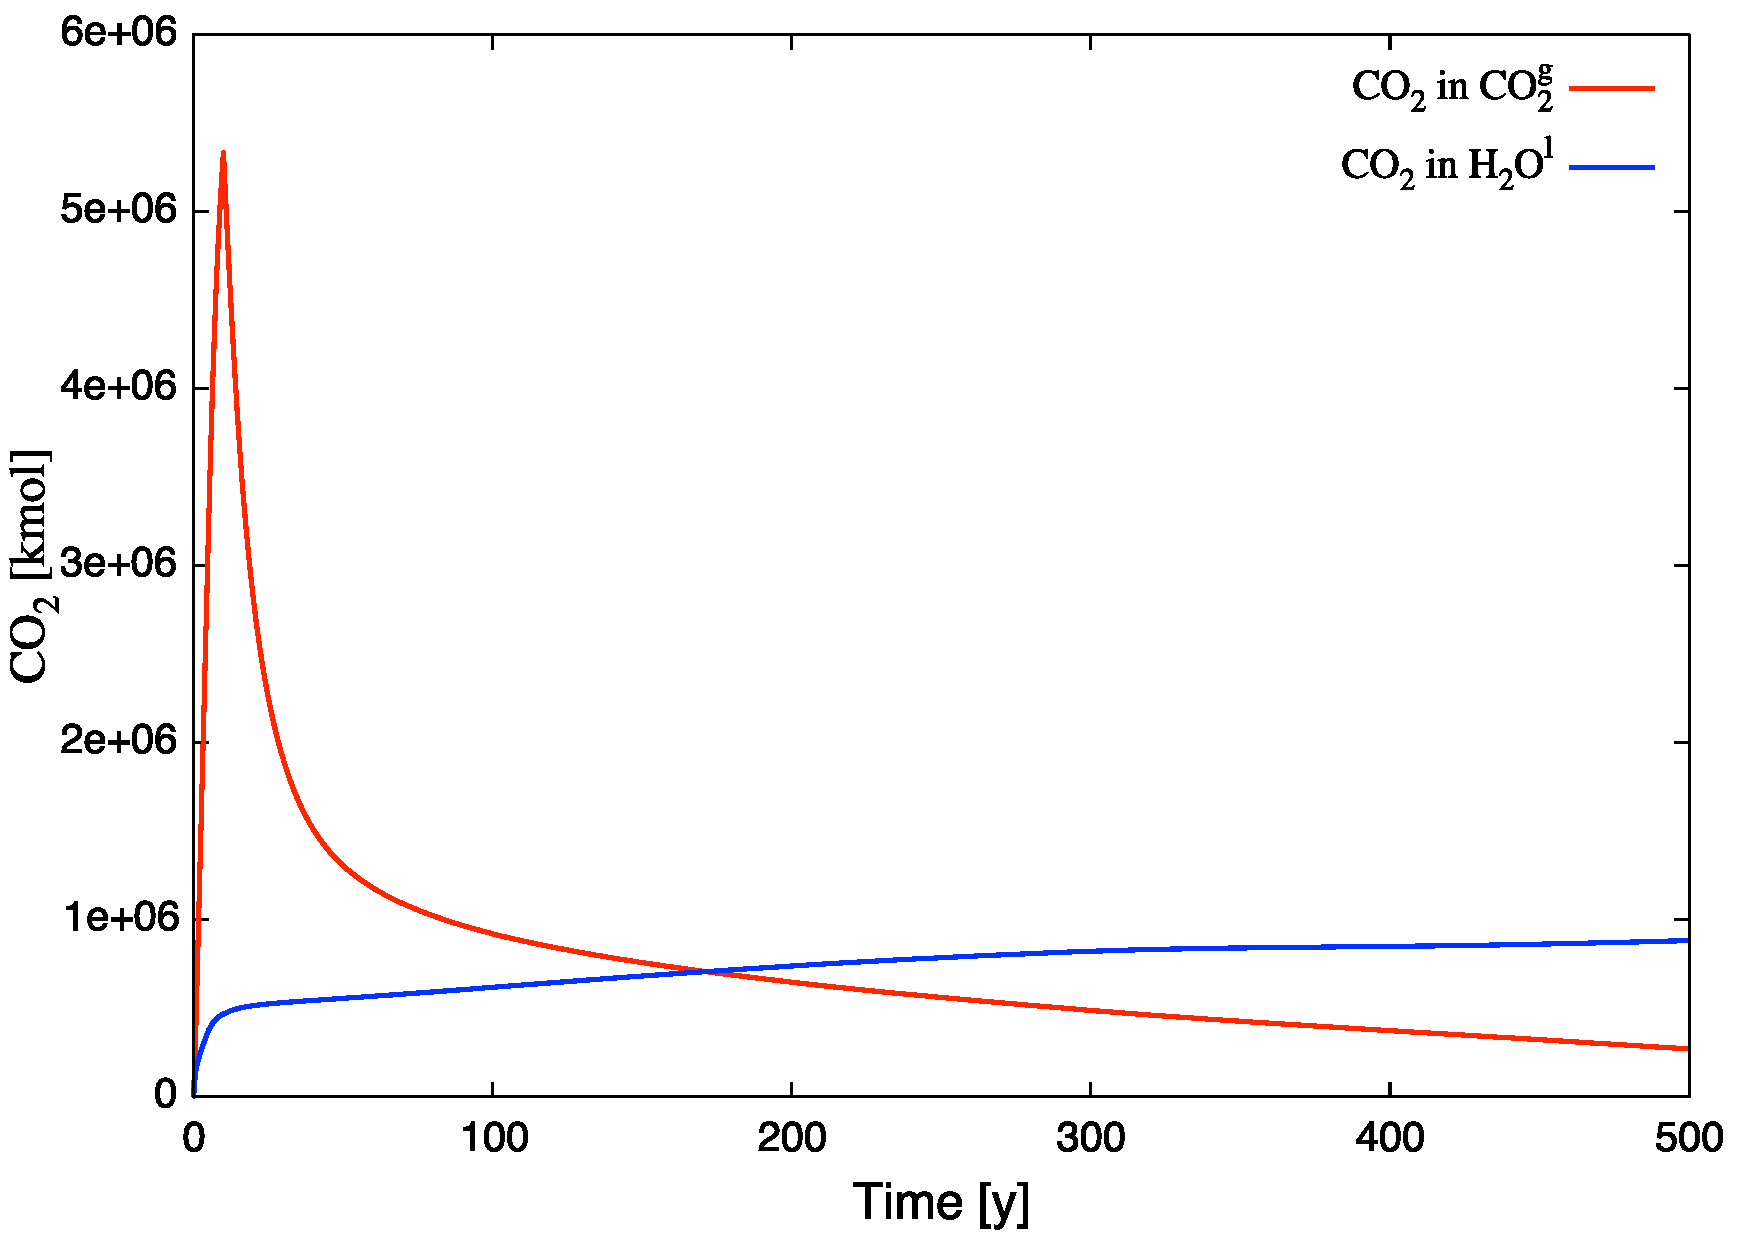
\includegraphics[scale=0.45]{./figs/mass}
\caption{Moles of CO$_2$ as a function of time in H$_2$ and supercritical CO$_2$ phases.}\label{fmass}
\end{figure}

\begin{figure}\centering
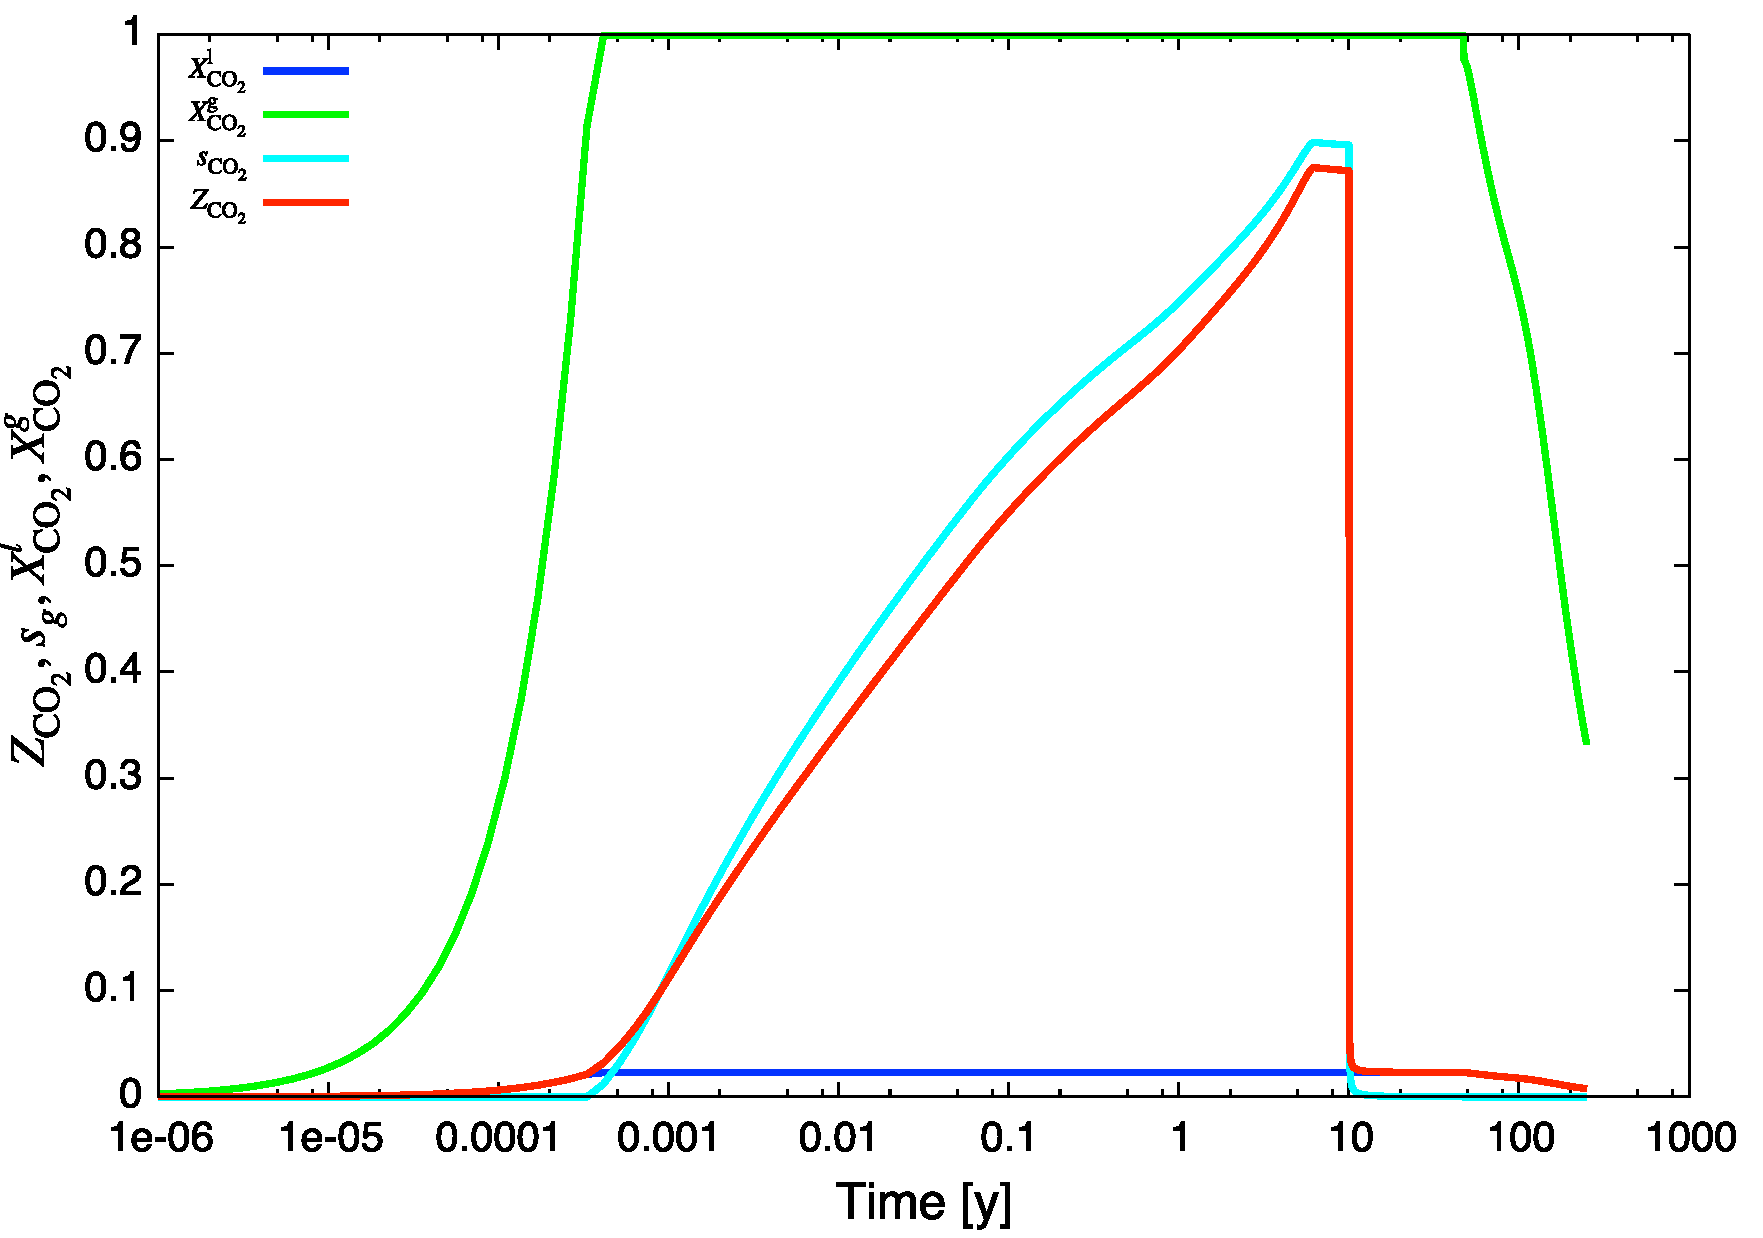
\includegraphics[scale=0.45]{./figs/zco2}
\caption{Plot showing $Z_\c$, $s_g$, $X_\c^l$ and $X_\c^g$ as functions of time at the injection well. The total mole fraction $Z_\c$ is piecewise continuous with a change in slope at phase changes and when the CO$_2$ saturation reaches the residual saturation.}\label{fzco2}
\end{figure}

\newpage
\section{References}
\begin{description}
\item Brooks, R.H. and A.T. Corey (1966) Properties of porous media affecting fluid flow, J. Irrig. Drain. Div., Am. Soc. Civil Eng. 92, 61--88.

\item Duan Z., and Sun, R. (2003) An improved model calculating CO2 solubility in pure water and aqueous NaCl solutions from 273 to 533 K and from 0 to 2000 bar, Chemical Geology 193, 257--271.

\item Duan, Z., Hu, J., Li, D., and Mao, S. (2008) Densities of the CO$_2$-H$_2$O and CO$_2$-H$_2$O-NaCl Systems up to 647 K and 100 MPa, Energy \& Fuels, 22, 1666--1674.

\item IAPWS, Revised Release on the IAPS Formulation 1985 for the Viscosity of Ordinary Water Substance, International Association for the Properties of Water and Steam, Erlangen, Germany, 1997, 15.

\item Kestin, J., Sengers, J.V., Kamgar-Parsi, B., Levelt Sengers, J.M.H. (1984) Thermophysical Properties of Fluid H$_2$O, J. Phys. Chem. Ref. Data, 13, 1, 175--183.

\item Li D., and Duan, Z. (2007) The speciation equilibrium coupling with phase equilibrium in the H$_2$O-CO$_2$-NaCl system from 0 to 250 $^\circ$C, from 0 to 1000 bar, and from 0 to 5 molality of NaCl, Chemical Geology 244, 730--751.

\item Span, R., Wagner, W. (1996) A New Equation of State for Carbon Dioxide Covering the Fluid Region from the Triple-Point Temperature to 1100 K at Pressures up to 800 MPa, J. Phys. Chem. Ref. Data, 25, 6, 1509--1596.

\item Revised Release on the IAPS Formulation 1985 for the Thermal Conductivity of Ordinary Water Substance, International Association for the Properties of Water and Steam, London, 1998, 23. 

\item van Genuchten, M.T.H. (1980) A closed form equation for redicting the hydraulic conductivity of unsaturated soils, Soil Sci. Soc. Am. J., 44, 892--898.

\end{description}

%\bibliographystyle{plainnat}
%\bibliography{./reference-new}
\clearpage

\section*{Appendix A: Composition Variables}
\addcontentsline{toc}{section}{\protect\numberline{}{Appendix A: Composition Variables}} 


\renewcommand{\theequation}{A-\arabic{equation}}
\setcounter{equation}{0}

There are several different approaches possible for solving the governing multiphase-multicomponent flow and transport equations depending on the choice of independent variables. The total number of independent variables is determined by the Gibbs phase rule. 
For a nonisothermal system derived from $N_P$ single fluid phases\symbolfootnote[2]{For a system with $N_P$ pure phases (e.g. $l$, $g$), there are $2^{N_P}\!-\!1$ possible phase combinations  (e.g. $l$, $g$, $lg$).} (e.g. $l$, $g$) and $N_C$ components (e.g. H$_2$O, CO$_2$), there are $N_C+1$ independent variables or degrees of freedom including temperature. 
Note that the number of degrees of freedom is independent of the number of  phases that are present in the system. To see this, the variables representing the system and the constraints imposed on them are listed in Table~\ref{tdof}.

\begin{table}[h]\centering
\caption{Variables and constraints in a multiphase-multicomponent system.}
\label{tdof}

\vspace{3mm}
%\renewcommand{\tabcolsep}{1cm}
\renewcommand{\arraystretch}{1.25}
\begin{tabular}{lcccc}
\toprule
Variable & Symbol & Number of & Number of & Constraint Condition\\
&&Variables&Constraints&\\
\midrule
Temperature & $T$ & 1 & 0 & ---\\
Pressure & $P_\a$ & $N_P$ & $N_P\!-\!1$ & $P_{c,\a\b} = P_\b - P_\a$\\
Saturation & $s_\a$ & $N_P$ & 1 & $\sum_\a s_\a=1$\\
Mole Fraction & $X_i^\a$ & $N_P N_C$ & $N_P$ & $\sum_i X_i^\a=1$\\
---&---& --- & $N_C(N_P\!-\!1)$ & $\mu_i^\a = \mu_i^\b$\\
\midrule
Total: && $N_P(N_C+2)+1$ & $N_P (N_C + 2)-N_C$\\
\midrule
Net: && \multicolumn{2}{c}{$N_C+1$}\\
\bottomrule
\end{tabular}
\end{table}

For any particular control volume the quantity $n_i^\a$, equal to the number of moles of the $i$th component in phase $\a$, completely determines the chemical composition of the system. The total number of moles in phase $\a$, $n_\a$ is obtained by summing $n_i^\a$ over all components:
\EQ
N_\a \eq \sum_i n_i^\a.
\EN
The total number of moles in the system is then
\EQ
N \eq \sum_\a N_\a.
\EN
The mole fraction $X_i^\a$ of the $i$th species relative to phase $\a$ is thus defined as
\EQ\label{sumx}
X_i^\a \eq \frac{n_i^\a}{N_\a}, \ \ \ \ \ \ \ \sum_i X_i^\a =1.
\EN
Other composition variables may also be defined and are useful to what follows. The phase mole fraction $\zeta_\a$ is defined as
\EQ
\zeta_\a \eq \frac{N_\a}{N} \eq \dfrac{\displaystyle\sum\limits_i n_i^\a}{\displaystyle\sum_{i'\a'} n_{i'}^{\a'}}, \ \ \ \ \ \ \ \sum_\a \zeta_\a =1.
\EN
The total component mole fraction $Z_i$ is defined by
\EQ\label{sumzi}
Z_i \eq \frac{N_i}{N} \eq \dfrac{\displaystyle\sum_\a n_i^\a}{\displaystyle\sum_\a n_\a}, \ \ \ \ \ \ \ \sum_i Z_i=1.
\EN
These quantities are related by the expression
\EQ
Z_i \eq \frac{1}{N}\sum_\a n_i^\a \eq \sum_\a \frac{n_i^\a}{N_\a} \frac{N_\a}{N} \eq\sum_\a \zeta_\a X_i^\a.
\EN
It follows from the definition of $Z_i$ that
\EQ\label{zi}
Z_i \eq \dfrac{\displaystyle\sum_\a s_\a \rho_\a X_i^\a}{\displaystyle\sum_{\a} s_\a \rho_\a},
\EN
with molar density $\rho_\a$ and fluid volume fraction $s_\a$ for phase $\a$. The quantity $s_\a$ is defined as the ratio of fluid volume $V_\a$ of phase $\a$ to pore volume $V_p$
\EQ
s_\a \eq \frac{V_\a}{V_p},
\EN
and satisfies the relation
\EQ
\sum_\a s_\a \eq 1.
\EN
The pore volume $V_p$ is equal to the sum of all fluid phase volumes $V_\a$
\EQ
V_p \eq \sum_\a V_\a.
\EN
Eqn.\eqref{zi} then follows from the relations
\begin{subequations}
\BA
\frac{n_i^\a}{V} &\eq \frac{n_i^\a}{N_\a}\frac{N_\a}{V_\a}\frac{V_\a}{V_p}\frac{V_p}{V},\\
&\eq \varphi s_\a \rho_\a X_i^\a,
\EA
\end{subequations}
and
\begin{subequations}
\BA
\frac{N_\a}{V} &\eq \frac{N_\a}{V_\a}\frac{V_\a}{V_p}\frac{V_p}{V},\\
&\eq \varphi s_\a \rho_\a.
\EA
\end{subequations}
The formulation of the mass conservation equations in terms of $Z_i$ as a presistent variable is used in the FLASH approach to avoid the necessity for variable switching.

Note that for a system consisting of a single phase, the expression for $Z_i$ reduces to
\EQ
Z_i \eq X_i^\a, \ \ \ \ \ \text{(pure phase $\a$)},
\EN
according to Eqn.\eqref{zi}.

\renewcommand{\theequation}{B-\arabic{equation}}
\setcounter{equation}{0}

\section*{Appendix B: Constitutive Relations}
\addcontentsline{toc}{section}{\protect\numberline{}{Appendix B: Constitutive Relations}} 

\renewcommand{\thesubsection}{B-\arabic{subsection}}
\setcounter{subsection}{0}

\subsection{Material Properties}

Material fluid properties for density, viscosity, internal energy and enthalpy are needed for pure H$_2$O and supercritical CO$_2$, and in the case of nonisothermal systems internal energy and enthalpy. In addition, mixture properties for CO$_2$ dissolved in H$_2$O and H$_2$O dissolved in supercritical CO$_2$ are needed. 
Each phase $\a$ is a mixture of species H$_2$O and CO$_2$. 
%For H$_2$O, $W_{\rm H_2O} = 18.01534$ kg/mol, and for CO$_2$, $W_{\c} = 44.0098$ kg/kmol.


\subsubsection{Pure H$_2$O}

The density, viscosity, internal energy, and enthalpy of pure H$_2$O are taken from the steam tables [International Formulation Committee of the Sixth International Conference on Properties of Steam, (1967)] and is valid for the pressure and temperature range of $0 \!<\! P \!<\! 1000$ bars, and $0 \!<\! T \!<\! 800$\degc. In addition, the saturation curve of H$_2$O, $P_{\rm sat}(T)$ and its inverse relation $T_{\rm sat}(P_v)$, for vapor pressure $P_v$, are also provided.

\noindent
Critical temperature ($T_c$) 373.946\degc\\
Critical pressure ($P_c$) 220.640 bar\\
Critical density ($\rho_c$) 322.000000 kg/m$^3$\\
$W_{\rm H_2O} = 18.01534$ kg/mol

\subsubsection{Supercritical CO$_2$}

Material properties of supercritical CO$_2$ are obtained from an equation of state such as Span and Wagner (1996) for density, viscosity, internal energy, enthalpy, fugacity, and fugacity coefficient as functions of temperature and pressure.

\noindent
Critical temperature: ($T_c$) 30.9782\degc\\
Critical pressure: ($P_c$)	73.773 bar\\
Critical density: ($\rho_c$) 467.600 kg/m$^3$\\
$W_{\c} = 44.0098$ kg/kmol

\subsubsection{Mixture Properties}

The mixture density for CO$_2$ dissolved in H$_2$O (liquid phase) is derived from Duan et al. (2008). For supercritical CO$_2$ a mixture density is not needed because of the low concentration of H$_2$O in the supercritical CO$_2$ phase.

\subsection{Capillary Pressure}

The pressure $P_\a$ of fluid phase $\a$ is related to the fluid pressure of phase $\b$ through the capillary pressure $P_{\a\b}^c$
\EQ\label{pc}
P_{\a\b}^c \eq P_\b - P_\a,
\EN
where $P_\b$ is assumed to be the non-wetting phase, in this case supercritical CO$_2$, and $P_\a$ refers to the wetting phase in this case brine. Capillary pressure is related to saturation $s_\a$ using, for example, van Genuchten or Brooks-Cory correlations.

\subsubsection{van Genuchten Relations}

Irreducible liquid saturation described by the van Genuchten (1980) relation is given by
\EQ\label{seff}
s_e \eq \left[1+\left( \alpha |P_c| \right)^n \right]^{-m}, 
\EN 
where $P_c$ [Pa] represents the capillary pressure, $\a$ [Pa$^{-1}$] is a parameter, and the effective liquid saturation $s_e$ is defined by 
\EQ 
s_e \eq \frac{s_l^{} - s_l^r}{s_l^0 - s_l^r}, 
\EN 
where $s_l^{}$ denotes liquid saturation, $s_l^r$ denotes the residual saturation, and $s_l^0$ denotes the maximum saturation. The constants $n$ and $m$ are related by the expressions 
\EQ\label{lambda} 
m \eq 1-\frac{1}{n}, \ \ \ \ \ n \eq \frac{1}{1-m}. 
\EN 
The inverse relation is given by
\EQ
P_c \eq \frac{1}{\alpha} \left[\left(s_e\right)^{-1/m} -1 \right]^{1/n}.
\EN
The derivative of $P_c$ with respect to saturation is given by
\EQ
\frac{dP_c}{ds_e} \eq -\frac{P_c}{nm} \dfrac{s_e^{-(1+1/m)}}{s_e^{-1/m}-1}.
\EN

The relative permeability for the liquid phase is given by
\EQ\label{krl} 
k_{rl} \eq \sqrt{s_e} \left\{1-\left[1-s_e^{1/m} \right]^m \right\}^2, 
\EN 
and for the gas phase by
\EQ 
k_{rg} \eq 1 - k_{rl}.
\EN 
Note that $k_{rl}$ = 0 for saturations below the residual saturation. 
The derivative of $k_{rl}$ with respect to saturation is given by
\EQ
\frac{dk_{rl}}{ds_e} \eq \frac{1}{2} \frac{k_{rl}}{s_e} + 2 \sqrt{s_e}
\left\{1-\left[1-s_e^{1/m} \right]^m\right\}
\left[1-s_e^{1/m} \right]^{m-1} s_e^{1/m-1}.
\EN

\subsubsection{Brooks-Corey Relations}

Irreducible liquid saturation described by the Brooks-Corey (1966) relation 
\EQ\label{seffbc}
s_e \eq \left( \alpha |P_c| \right)^{-\lambda}, 
\EN 
with the inverse relation given by
\EQ
P_c \eq \frac{1}{\alpha} \left(s_e\right)^{-1/\lambda}.
\EN
The derivative of $P_c$ with respect to saturation is given by
\EQ
\frac{dP_c}{ds_e} \eq -\dfrac{P_c}{\lambda s_e}.
\EN

The relative permeability function is given by 
\BA 
k_{rl} &= \left(s_e \right)^{(2+3\lambda)/\lambda},\nonumber\\
&= \left( \alpha |P_c| \right)^{-(2+3\lambda)}, \label{krlbc}
\EA 
for the liquid phase, and for the gas phase as
\EQ 
k_{rg} \eq 1 - k_{rl}.
\EN 
Note that $k_{rl}$ = 0 for saturations below the residual saturation. 
The derivative of $k_{rl}$ with respect to saturation is given by
\EQ
\frac{dk_{rl}}{ds_e} \eq \frac{2+3\lambda}{\lambda} \dfrac{k_{rl}}{s_e}.
\EN

\subsubsection{Linear}

\subsection{Interface Properties}

Shown in Table~\ref{tinterface} is the interface averaging assumption made for each quantity listed.

\begin{table}[h]\centering
\caption{Interface Property}\label{tinterface}

\vspace{3mm}

\renewcommand{\arraystretch}{2}
\begin{tabular}{lccc}
\toprule
Property & Symbol(s) & Average & Expression\\
\midrule
Permeability & $k$ & Harmonic & $\dfrac{k_1 k_2(d_1+d_2)}{d_1 k_2 + d_2 k_1}$\\
\midrule
Mole Fraction & $Z_i$ & Upwinding & $Z_{i,nn'} = Z_{in}, \ q_{nn'}>0$\\
&&&$Z_{i,nn'} = Z_{in'}, \ q_{nn'}<0$ \\
\midrule
Density & $\rho_\a$ & Arithmetic & $\dfrac{d_2\rho_2 + d_1\rho_1}{d_1+d_2}$\\
\midrule
Diffusion & $s_\a\tau_\a D_\a$ & Harmonic & $\dfrac{(s_\a\tau_\a D_\a)_1(s_\a\tau_\a D_\a)_2 (d_1+d_2)}{d_2(s_\a\tau_\a D_\a)_1 + d_1(s_\a\tau_\a D_\a)_2}$\\
\bottomrule
\end{tabular}
\end{table}


\section*{Appendix C: Supercritical CO$_2$--H$_2$O Equilibrium Relations}
\label{sec:eqrel}
\addcontentsline{toc}{section}{\protect\numberline{}{Appendix C: Supercritical CO$_2$--H$_2$O Equilibrium Relations}} 
\renewcommand{\theequation}{C-\arabic{equation}}
\setcounter{equation}{0}

For an aqueous fluid in equilibrium with supercritical CO$_2$ it is necessary to use an equation of state for CO$_2$ to obtain the solubility of CO$_2$ in solution. The presentation follows Duan and Sun (2003). 

Equilibrium of supercritical CO$_2$ with an aqueous solution is described by the reactions
\begin{subequations}
\EQ\label{co2}
{\rm CO}_2^l \arrows {\rm CO}_2^g,
\EN
and
\EQ\label{h2o}
{\rm H_2O}^l \arrows {\rm H_2O}^g.
\EN
\end{subequations}
The mass action equation corresponding to reaction \eqref{co2} is given by
\EQ\label{massactco2}
K_\c^{\rm eq} \eq \frac{f_\c^{}}{a_\c^{\rm eq}} 
\eq \frac{\phi_\c^{} P_\c^g}{a_\c^{\rm eq}} 
\eq \frac{\phi_\c^{} X_\c^g P_g^{}}{a_\c^{\rm eq}},
\EN
with equilibrium constant $K_\c^{\rm eq}$.
The activity of $\c$ in the aqueous solution is related to its molality $m_\c^{\rm eq}$ by
\EQ
a_\c^{\rm eq} \eq \gamma_\c^{\rm eq} m_\c^{\rm eq},
\EN
where $\gamma_\c$ denotes the activity coefficient.
The fugacity is given by
\EQ
f_\c^{} \eq \phi_\c^{} P_\c^{g} \eq \phi_\c^{} X_\c^g P_g^{},
\EN
with fugacity coefficient $\phi_\c$, where the equilibrium mole fraction of $\c$ in the supercritical (gas) phase, $X_\c^{g,\rm eq}$, is assumed to be given by
\EQ\label{xco2g}
X_\c^{g,\rm eq} \eq \frac{P_\c^g}{P_g} \eq \frac{P_g-P_\w^{\rm sat}(T)}{P_g} \eq 1-\frac{P_\w^{\rm sat}(T)}{P_g},
\EN
with total gas pressure $P_g$ equal to
\EQ\label{totalp}
P_g \eq P_\c^g + P_\w^{\rm sat}(T),
\EN
and where $P_\w^{\rm sat}(T)$ denotes the saturation pressure of pure water. 
The equilibrium concentration of CO$_2$ in the aqueous solution in terms of molality units is thus given by
\EQ\label{m_to_x}
m_\c^{\rm eq} \eq \frac{\phi_\c^{} X_\c^g}{\gamma_\c^{}K_\c^{\rm eq}}  P_g^{}.
\EN
Molality is related to mole fraction $X_\c^{l,{\rm eq}}$ by the equation
\begin{subequations}
\EQ\label{xco2l}
X_\c^{l,{\rm eq}} \eq\frac{W_\w m_\c^{\rm eq}}{1 + W_\w m_\c^{\rm eq}},
\EN
and conversely mole fraction is related to molality by the inverse relation
\EQ
m_\c^{\rm eq} \eq \frac{X_\c^{l,{\rm eq}}}{W_\w(1-X_\c^{l,{\rm eq}})},
\EN
\end{subequations}
where $W_\w$ denotes the formula weight of water. Substituting Eqn.\eqref{m_to_x} gives
\EQ
X_\c^l \eq \frac{W_\w \widetilde K_\c^{} \big(P_g-P_w^{\rm sat}(T)\big)}{1+W_\w \widetilde K_\c^{} \big(P_g-P_w^{\rm sat}(T)\big)},
\EN
using Eqn.\eqref{xco2g}, where
\EQ
\widetilde K_\c \eq \big(K_\c^{\rm eq}\big)^{-1} \frac{\phi_\c}{\gamma_\c}.
\EN
The derivative with respect to pressure $P_g$ needed to construct the Jacobian matrix is given approximately by
\EQ
\frac{\p X_\c^l}{\p P_g} \eq \frac{W_\w \widetilde K_\c^{}}{\left(1+W_\w \widetilde K_\c^{} \big(P_g-P_w^{\rm sat}(T)\big)\right)^2}.
\EN
This expression ignores the derivative of the fugacity coefficient $\phi_\c$.

\section*{Appendix D: Phase Change Criteria}
\addcontentsline{toc}{section}{\protect\numberline{}{Appendix D: Phase Change Criteria}} 

\renewcommand{\theequation}{D-\arabic{equation}}
\setcounter{equation}{0}


In the FLASH approach the primary variables are $P$, $T$ and the total mole fraction $Z_i$ of the $i$th component summed over all phases.
This gives $2+N_C-1 = N_C+1$ independent variables as required. The variable $Z_i$ is a persistent degree of freedom throughout the simulation. From the knowledge of $Z_i$ it is possible to obtain the stable phase assemblage, the volume fraction $s_\a$ of each phase present in the system, and its composition in terms of $X_i^\a$ as indicated in Table~\ref{tphase}. 

\begin{table}[h]\centering
\caption{Phase Transition}
\label{tphase}

\vspace{3mm}

\renewcommand{\arraystretch}{1.5}
\begin{tabular}{cc}
\toprule
Region & Stable Phase(s)\\
\midrule
$Z_\c^{} \leq X_\c^{l,\rm eq}$ & liquid\\
$X_\c^{l,\rm eq} < Z_\c^{} < X_\c^{g,\rm eq}$ & two-phase\\
$X_\c^{g,\rm eq} \leq Z_\c^{}$ & gas\\
\bottomrule
\end{tabular}
\end{table}

For a two-phase ($\a=l$, $\sc$) system where, for example, $l$ designates the liquid phase $\w$ and $\sc$ designates supercritical $\c$, $Z_i$ can be expressed as
\EQ\label{zisg}
Z_i \eq \frac{\rho_l^{} s_l^{} X_i^l + \rho_{\sc}^{} s_{\sc}^{} X_i^{\sc}}{\rho_l^{} s_l^{} + \rho_{\sc}^{} s_{\sc}^{}},
\EN
for molar fluid densities $\rho_l$, $\rho_{\sc}$ and phase saturation $s_l$, $s_{\sc} \!=\! 1\!-\!s_l$.
Solving this equation for $s_g$ gives
\EQ\label{sg}
s_g \eq \frac{\rho_l^{} (Z_i^{}-X_i^l)}{\rho_l^{} (Z_i^{} - X_i^l) - \rho_g^{} (Z_i^{} -X_i^g)}, \ \ \ \ \ (i= {\rm H_2O,\, CO_2}).
\EN

One has for the derivatives of $s_g (P,\, T,\,Z)$:
\begin{subequations}
\BA
s_{gZ}^{} & \eq \frac{\p s_g}{\p Z},\\
& \eq \frac{\rho_l^{}\rho_g^{} (X_i^g - X_i^l)}{\rho_l^{}(Z-X_i^l) - \rho_g^{}(Z-X_i^g)},
\EA
\end{subequations}
\begin{subequations}
\BA
s_{gP}^{} &\eq \frac{\p s_g}{\p P},\\
& \eq \frac{Z_i-X_i^l}{D}\left[\rho_{lP}^{} - \frac{\rho_l}{D}\left(\rho_{lP}^{}(Z_i-X_i^l) - \rho_{gP}^{} (Z_i-X_i^g)\right)\right]\nonumber\\
&\qquad -\frac{\rho_l}{D} \left[X_{iP}^l - \frac{Z_i-X_i^l}{D}\left( \rho_l^{} X_{iP}^l - \rho_g^{} X_{iP}^g \right)
\right],
\EA
\end{subequations}
where
\EQ
D \eq \rho_l^{} (Z_i^{} - X_i^l) - \rho_g^{} (Z_i^{} -X_i^g).
\EN

For single phase liquid or gas systems it follows that Eqn.\eqref{zisg} reduces to
\EQ
Z_i \eq X_i^\a, \ (\a=l,\,g),
\EN
and 
\EQ
s_g \eq \left\{
\begin{array}{ll}
1 & \a=g\\
0 & \a=l
\end{array}\right..
\EN

To determine the mole fractions $X_i^\a$ from $Z_i$ it is necessary to consider the equilibrium constraints between phases expressed as equality their chemical potentials in the two phases.
Depending on the value of $Z_\c$ different phases are present in the system (see Table~\ref{tphase}).
\begin{description}
\item[Single Liquid Phase:] For $Z_\c \!\leq\! X_\c^{l,{\rm eq}}$, a single aqueous ($\w$) phase is the stable phase assemblage.
The aqueous $\c$ concentration is equal to
\begin{subequations}\label{fla-sec-c1}
\BA\label{liq}
X_i^l = Z_i^{},
\EA
and phase saturations are given by
\BA
s_l = 1, \ s_{\sc} =0,
\EA
\end{subequations}
consistent with Eqn.\eqref{sg}.

\item[Single Gas Phase:] For $Z_\c\!\geq\! X_\c^{g,\rm eq} \!=\!1\!-\!P_\w^{\rm sat}(T)/P_g$, a single supercritical $\c$ phase is the stable phase assemblage.
The supercritical $\c$ concentration is equal to
\begin{subequations}\label{fla-sec-c2}
\BA\label{gas}
X_i^{\sc} = Z_i^{},
\EA
and phase saturations are given by
\BA
 s_l = 0, \ s_{\sc} =1,
\EA
\end{subequations}
consistent with Eqn.\eqref{sg}.

\item[Two-Phase:] For $X_\c^{l,{\rm eq}} \!<\! Z_\c \!<\! X_\c^{g,{\rm eq}}\!=\!1\!-\!P_\w^{\rm sat}/P_g$, the two phases supercritical $\c$ and a liquid phase coexist.
From Section \ref{sec:eqrel} the equilibrium mole fractions of CO$_2$ in the liquid and gas phases are given by Eqns.\eqref{xco2l} and \eqref{xco2g}, respectively.
Note that the equilibrium composition only depends on temperature and pressure and is independent of $Z_\c$, and thus forms an invariant composition. The gas saturation is determined from Eqn.\eqref{sg}
\EQ\label{2ph}
s_{\sc} \eq \frac{\rho_{l}^{} (Z_{\c}^{} - X_{\c}^{l,\rm eq})}
{\rho_l^{} (Z_{\c}^{} - X_{\c}^{l,\rm eq}) - \rho_{\sc}^{} (Z_{\c}^{} - X_{\c}^{\sc,\rm eq})},
\EN
with $s_l\!=\!1\!-\!s_{\sc}$.
The densities of the aqueous and supercritical $\c$ phases are obtained from an equation of state, as a function of $P$, $T$ and $X_i^{l,\,g}$, based on the mixture rules for the phase.
\end{description}

\end{document}

========================================================================
========================================================================

Activity coefficients and standard state potentials are related by
\BA
\mu_i &\eq \mu_i^m + RT \ln \gamma_i m_i,\\
&\eq \mu_i^x + RT \ln \lambda_i x_i,
\EA
with [see Denbigh (1981), p. 278, Eqns.(9$\cdot$19) and (9$\cdot$20)]
\EQ
\gamma_i \eq x_w \lambda_i,
\EN
and
\EQ
\mu_i^m \eq \mu_i^x + RT \ln W_w.
\EN

The concentration of $\c$ in the gas phase, $C_\c^g$, is obtained as
\BA
C_\c^g &\eq \frac{n_i^g}{V_g} \eq \frac{n_i^g}{N_g}\frac{N_g}{V_g} \eq \rho_\c^{} X_\c^g,\\
&\eq \rho_\c \frac{f_\c}{\phi_\c P_g},\\
&\eq \rho_\c K_\c^{\rm eq} \frac{a_\c}{\phi_\c P_g}.
\EA


In the general case molality and mole fraction of solute species $i$ are related by the expressions
\EQ
m_i \eq \frac{x_i}{W_w x_w} \eq \frac{x_i}{W_w(1-\sum_{l\ne w} x_l)},
\EN
and the inverse relation
\EQ
x_i \eq \frac{W_w m_i}{1+W_w \sum_{l\ne w} m_l},
\EN
where $x_w$ and $W_w$ denote the mole fraction and formula weight of the solvent, in this case $\w$, respectively, with
\EQ
x_w \eq \frac{1}{1+W_w \sum_{l\ne w} m_l}.
\EN

implies equality of the chemical potentials
\EQ
\mu_\c^l \eq \mu_\c^g,
\EN
where
\EQ
\mu_\c^l \eq \mu_\c^{\ominus l} + RT\ln a_\c^{},
\EN
and
\EQ
\mu_\c^g \eq \mu_\c^{\ominus g} + RT\ln f_\c^{},
\EN
with standard state chemical potentials $\mu_\c^{\ominus l}$ and $\mu_\c^{\ominus g}$. The activity of $\c$ in an aqueous solution is related to its molality $m_\c$ by
\EQ
a_\c^{} \eq \gamma_\c^{} m_\c^{},
\EN
where $\gamma_\c$ denotes the activity coefficient for aqueous $\c$.
The fugacity is given by
\EQ
f_\c^{} \eq \phi_\c^{} P_\c^{} \eq \phi_\c^{} X_\c^g P_g^{},
\EN
with fugacity coefficient $\phi_\c$ where the mole fraction of $\c$ in the supercritical (gas) phase, $X_\c^g$, is assumed to be given by
\EQ
X_\c^g \eq \frac{P_\c^g}{P_g} \eq \frac{P_g-P_\w^{\rm sat}(T)}{P_g} \eq 1-\frac{P_\w^{\rm sat}(T)}{P_g},
\EN
with total gas pressure $P_g$ equal to
\EQ\label{totalp}
P_g \eq P_\c^g + P_\w^{\rm sat}(T),
\EN
and where $P_\w^{\rm sat}(T)$ denotes the saturation pressure of pure water. 

Introducing the equilibrium constant $K_\c^{\rm eq}$ defined as
\EQ
\ln K_\c^{\rm eq} \eq -\frac{1}{RT}\big(\mu_{\rm CO_2}^{g\ominus} - \mu_{\rm CO_2}^{l\ominus}\big),
\EN
yields the mass action equation
\EQ\label{massactco2}
K_\c^{\rm eq} \eq \frac{f_\c^{}}{a_\c^{}} \eq \frac{\phi_\c^{} P_\c^g}{a_\c} \eq \frac{\phi_\c^{} X_\c^g P_g^{}}{a_\c^{}}.
\EN
The equilibrium CO$_2$ molality is thus given by
\EQ
m_\c^{} \eq \frac{\phi_\c^{} X_\c^g}{\gamma_\c^{}K_\c^{\rm eq}}  P_g^{}.
\EN
%Of the three quantities: $P_g$, $P_\c^g$, and $T$, two may be specified and the other computed from Eqn.\eqref{totalp}.
Solving Eqn.\eqref{massactco2} for the $\c$ partial pressure gives
\BA
P_\c^g &\eq \frac{K_\c^{\rm eq}}{\phi_\c} a_\c,\\
&\eq \widetilde K_\c^{\rm eq} a_\c,
\EA
where the effective equilibrium constant $\widetilde K_\c$ is defined as
\EQ
\widetilde K_\c^{\rm eq} \eq \frac{K_\c^{\rm eq}}{\phi_\c}.
\EN

For a two-component system $\w$, $\c$, molality is related to the mole fraction by the equation
\begin{subequations}
\EQ
x_\c^l \eq\frac{W_\w m_\c}{1 + W_\w m_\c},
\EN
and conversely mole fraction is related to molality by the inverse relation
\EQ
m_\c \eq \frac{x_\c^l}{W_\w(1-x_\c^l)},
\EN
\end{subequations}
where $W_\w$ denotes the formula weight of water. 

\BA
R_{in}^{k+1} \eq &\sum_\a \left\{\frac{\big(\varphi s_\a \rho_\a X_i^\a\big)_n^{k+1}-(\varphi s_\a \rho_\a X_i^\a)_n^k}{\Delta t_{k+1}} \right\} V_n \nonumber\\
& + \sum_{\a n'} (F_i^\a )_{nn'}^{k+1} A_{nn'} \nonumber\\
&- Q_{in}^{k+1} V_n,
\EA


\subsubsection{Two-Component System}

\begin{comment}
One important assumption in the implementation in PFLOTRAN is that the activity coefficients in the aqueous phase and the fugacity coefficient in the supercritical phase are not functions of the $\c$ concentration. 
%I.e. non-ideality is weak in the aqueous and gas mixtures. 
This assumption is consistent with the solubility equations for $\c$ [\cite {garcia01}, \cite{duan2003}, \cite{duan2008}] adapted in PLOTRAN. With this assumption, the phase distribution parameters $K_i(P,\,T)$ are not functions of the mole fractions $z_i, x_i$ and $y_i$, which greatly simplifies the Flash calculation. 
\end{comment}

Currently the FLASH2 mode in PFLOTRAN can only handle systems with two components and two phases, enabling the Flash calculation to be carried out in a simplified manner. 
For a two-component system the FLASH equations may be solved analytically. 
In this case, with the notation $x_i = X_i^l$ and $y_i = X_i^g$, there are four constraint conditions in four unknowns ($x_1,\,x_2,\,y_1,\,y_2$):
\begin{subequations}
\EQ
y_i=K_ix_i,
\EN
\EQ
x_1+x_2\eq 1,
\EN
and
\EQ
y_1+y_2 \eq K_1 x_1 + K_2 x_2 \eq 1,
\EN
\end{subequations}
These equations have the solution
\begin{subequations}
\EQ
x_1 = \frac{1-K_2}{K_1-K_2}, \ \ \ x_2=1-x_1 \eq \frac{K_1-1}{K_1-K_2},
\EN
and
\EQ
y_1 = \frac{K_1(1-K_2)}{K_1-K_2}, \ \ \ y_2 \eq \frac{K_2(K_1-1)}{K_1-K_2}.
\EN
\end{subequations}
The gas phase mole fraction $\zeta_g$ can then be obtained from the equation
\EQ
Z_i \eq (1-\zeta_g) x_i + \zeta_g K_i x_i,
\EN
to give
\begin{subequations}
\BA
\zeta_g &\eq \frac{Z_i - x_i}{(K_i-1)x_i}, \ \ \ \ \ (i=1,\,2),\\
&\eq \frac{Z_1(K_1-K_2)-(1-K_2)}{(K_1-1)(1-K_2)},\\
&\eq \frac{Z_2(K_1-K_2)-(K_1-1)}{(K_1-1)(1-K_2)}.
\EA
\end{subequations}

Both $K_1$ and $K_2$ are functions of $P$ and $T$. The quantity $K_2$, however, is also a function of $x_\c$. For the equilibrium relation for component $\w$ it is assumed that
\EQ
K_1 \eq \frac{P_{\rm sat}(T)}{P}.
\EN
The equilibrium relation for the $\c$ component is obtained from the mass action relation
\EQ
K_\c^{\rm eq} \eq \frac{\phi_\c y_\c P}{\gamma_\c m_\c}.
\EN
Solving for $m_\c$ gives
\EQ
m_\c \eq \frac{\phi_\c y_\c P}{K_\c^{\rm eq}\gamma_\c}.
\EN
Substituting the relation
\EQ
m_\c \eq \frac{x_\c}{W_\w(1-x_\c)},
\EN
gives
\EQ
y_\c \eq K_2 x_\c,
\EN
with
\EQ
K_2 \eq \frac{K_\c^{\rm eq}\gamma_\c}{W_\w(1-x_\c)\phi_\c P}.
\EN
Thus $K_2$ is a function of $x_\c$ yielding a quadratic equation for $x_\c$. 

Under conditions of thermodynamic equilibrium, liquid and gas mole fractions are related by a pseudo-equilibrium constant $K_i$, which may depend on composition, defined through the relation
\EQ\label{yi}
X_i^g \eq K_i^{} X_i^l. 
\EN
Let $\zeta_g$ represent the supercritical $\c$ phase mole fraction defined as
\EQ
\zeta_g\eq\frac{1}{N}\sum_i n_i^g.
\EN
%Under a phase transformation mass conservation implies the relation
The total mole fraction $Z_i$ simplifies to
\EQ
Z_i \eq \zeta_g X_i^g + (1-\zeta_g) X_i^l.
\EN
Using Eqn.\eqref{yi} it follows that
\EQ
Z_i \eq \zeta_g K_i X_i^l + (1-\zeta_g) X_i^l,
\EN
from which
\begin{subequations}\label{addphase_N2}
\BA
X_i^l \eq \frac{Z_i}{1+(K_i-1)\zeta_g}, 
\EA
and
\BA
X_i^g \eq \frac{K_i Z_i}{1+(K_i-1)\zeta_g}. 
\EA
\end{subequations}
The value of $\zeta_g$ can be found by solving the Flash equation (i.e. the Rachford-Rice equation)
\EQ\label{flash}
\F(\zeta_g)=\sum_i(X_i^g-X_i^l)=\sum_i \frac {Z_i(K_i-1)}{1+(K_i-1)\zeta_g} =0.
\EN
Eqn.(\ref{flash}) indicates that the Flash method is not applicable to a multiphase system with phase equilibrium distribution coefficients $K_i$ equal to unity, e.g. the water-steam system. Under such situations Eqn.(\ref{flash}) is trivially satisfied.

Since $\F(\zeta_g)$ is a monotonically decreasing function of $\zeta_g$, a meaningful solution $0\leq \zeta_g\leq 1$ can exist only if 
\begin{subequations}\label{addphase_N3}
\BA\label{liqbc}
\sum_i K_i Z_i \geq 1,
\EA
or
\BA\label{vapbc}
\sum_i \frac{Z_i}{K_i} \leq 1.
\EA
\end{subequations}
If the equality in Eqn.(\ref{liqbc}) is satisfied the gas phase is stable, whereas if the equality in Eqn.(\ref{vapbc}) is valid the liquid phase is stable. 
%These conditions were referred to by \cite{michelsen-2-1982} in his discussion on phase change calculations. 
%It was demonstrated that this criteria is consistent with the tangent plane method applied to the minimization of the Gibbs free energy [\cite{michelsen-1-1982}, \cite{nghiem-1985}]. A more detailed discussion can be found in these references. In the PFLOTRAN MPHASE mode in which variable switching is employed, the solution of Eqn.(\ref{flash}) for a single node is used as the initial guess for saturation for a phase transition from single to two phase, although the efficiency of this initial guess is not entirely satisfactory because the node does not represent a closed system.

Eqns.(\ref{addphase_N3}) a, b are used as criteria to determine the existence of a change in phase in the implementation of the Flash mode; i.e. if $\sum_i K_i Z_i \leq 1$, then only a liquid phase exists ($Z_{\rm H_2O}\!=\!1$); if $\sum_i {Z_i}/{K_i} \geq 1$, then only a gas phase exists ($Z_{\rm CO_2}\!=\!1$); otherwise two phases coexist ($0\!<\! Z_{\rm CO_2}\!<\!1$). Once the phase configuration (single aqueous phase, single supercritical phase, or coexisting two-phase system) is determined, the secondary variables are evaluated in the following steps. 

As stated previously, the coefficients $K_i$ are not functions of the $\c$ concentration. Their values at given $P$ and $T$ conditions are given explicitly by
\begin{subequations}
\BA
K_{\w} =\frac{P_{\w}^{\rm sat}(T)}{P},
\EA
and
\BA\label{k_value_c}
K_{\c} =\frac{H_{\c}\gamma_{\c}}{P\phi_{\c}}.
\EA
\end{subequations}
From these relations the phase composition can be obtained by solving a linear set of equation for the four unknown secondary variables $X_i^\alpha$, ($i$=H$_2$O, CO$_2$) and $\alpha=l$, $\sc$. One has
\EQ\label{k_value_w}
X_i^{\sc} = K_i X_i^l, \ \ \ (i = \w, \ \c),
\EN
From these results the phase densities $\rho_\alpha, \alpha=l$, $\sc$ can be calculated from $P$, $T$ and $X_i^\alpha$. Once the phase densities are obtained, the saturations $s_\alpha, \alpha=l$, $\sc$ can be obtained by solving the linear mass conservation equation
\EQ
\rho_l s_l X_{\c}^l + \rho_{\sc} s_{\sc} X_{\c}^{\sc} = (\rho_l s_l + \rho_{\sc} s_{\sc}) Z_{\c},
\EN 
with $s_l=1-s_{\sc}$ to give
\EQ\label{2ph}
s_{\sc} \eq \frac{\rho_{l} (Z_{\c} - X_{\c}^l)}
{\rho_l (Z_{\c} - X_{\c}^l) - \rho_{\sc} (Z_{\c} - X_{\c}^{\sc})}.
\EN


==============================================================

A common approach, referred to as variable switching is to select the independent variables at each control volume or grid cell dependent on the phases present. Several possibilities are listed in Table~\ref{tindepvar}. There exist $2^2\!-\!1=3$ possible phases in the system corresponding to liquid, gas and liquid-gas. In general for a system made up of $N_p$ individual phases, there are $2^{N_p}\!-\!1$ possible phase combinations.

An alternative approach is to use the so-called Flash method in which a persistent set of independent variables exit. This approach may be advantageous for use with multilevel solvers to avoid changing the independent variables on different levels within a patch.

In either case it is necessary to determine the stable phases present in a control volume based on conditions of thermodynamic equilibrium.

\tabcolsep 6pt
\begin{table}[H]\centering
\caption{Independent variables in a two-phase system.}\label{tindepvar}
\vspace{3mm}
\begin{tabular}{lccc}
\toprule
Phase & \multicolumn{3}{c}{Variables}\\
\midrule
liquid & $P_l$ & $T$ & $X_i^l$\\
gas & $P_g$ & $T$ & $X_i^g$\\
two-phase & $P_g$ & $T$ & $s_g$\\
& $P_g$ & $P_l$ & $s_g$\\
\bottomrule
\end{tabular}
\end{table}

Various constitutive relations hold depending on the phases present.

\subsubsection{Liquid Phase: Independent Variables $\{P_l,\,T,\,X_\c^l\}$}

For a pure liquid phase $s_l=1$. The molality of dissolved $\c$ is found from the relation
\EQ
m_\c^{l} \eq \frac{X_\c^l W_\w^{-1}}{1- X_\c^l - \displaystyle\sum_{i\ne \w,\c} \!\!\!\!\!\!X_i^l}.
\EN
with the inverse relation
\EQ
X_\c^l \eq \frac{m_\c  W_\w}{1 +  W_\w\big(m_\c + \displaystyle\sum_{i\ne \w,\c}\!\!\! \!\!\! m_i\big)}.
\EN

\subsubsection{Gas Phase: Independent Variables $\{P_g,\,T,\,X_\c^g\}$}

For a pure gas phase $s_g=1$.

\subsubsection{Two-Phase: Independent Variables $\{P_g,\,T,\,s_g\}$}

In a two-phase system
$X_\c^g$, is assumed to be given by
\EQ
X_\c^g \eq \frac{P_\c^g}{P_g} \eq \frac{P_g-P_\w^{\rm sat}(T)}{P_g} \eq 1-\frac{P_\w^{\rm sat}(T)}{P_g},
\EN
with total gas pressure $P_g$ equal to
\EQ
P_g \eq P_\c^g + P_\w^{\rm sat}(T),
\EN
and where $P_\w^{\rm sat}(T)$ denotes the saturation pressure of pure water. One also has
\EQ
X_\c^l = 1-X_\c^g. 
\EN
The molality of dissolved $\c$ is found from the relation
\EQ
m_\c^{} \eq \frac{\phi_\c^{} X_\c^g}{\gamma_\c^{}K_\c^{}} P_g^{}.
\EN

\subsection{Conditions for Change in Phase}

Possible changes in phase that may occur in the system are listed in Table~\ref{tphasechng}. In Table~\ref{tphasechng}, $\mu_i^\a$ refers to the chemical potential of the $i$th species in phase $\a$.

\begin{table}[H]\centering
\caption{Independent variables in a two-phase system.}\label{tphasechng}
\vspace{3mm}
\begin{tabular}{rclcrcl}
\toprule
\multicolumn{3}{c}{Phase Transformation} & Condition & \multicolumn{3}{c}{Variable Switching}\\
\midrule
liquid &$\rightarrow$& two-phase & $\mu_\c^l > \mu_\c^g$ & $\{P_l, \, T, X_\c^l\}$ &$\rightarrow$& $\{P_g, \, T, s_g\}$\\
gas &$\rightarrow$& two-phase & $\mu_\c^l < \mu_\c^g$ & $\{P_g, \, T, X_\c^g\}$ &$\rightarrow$& $\{P_g, \, T, s_g\}$\\
two-phase &$\rightarrow$& liquid & $s_g < 0$ & $\{P_g, \, T, s_g\}$ &$\rightarrow$& $\{P_g, \, T, X_\c^l\}$\\
two-phase &$\rightarrow$& gas & $s_g > 0$ & $\{P_g, \, T, s_g\}$ &$\rightarrow$& $\{P_g, \, T, X_\c^g\}$\\
\bottomrule
\end{tabular}
\end{table}

\subsection{Flash Method}

An alternative approach to variable switching is the Flash method.
Although the variable switching method is often considered stable and efficient, it has several shortcomings: 1) it causes perturbation during Newton iterations during phase changes; 2) the change in the definition of independent variables affects the structure of Newton-Raphson matrix; and 3) as a consequence this degrades performance of the preconditioner during the linear solve step. Finally, the variable switching approach is not appropriate for use with multilevel solvers because of the possibility for the need to solve for different independent variables on different levels.

\subsubsection{Two-Phase System}

An alternative to variable switching is to keep the primary variables preserved using the solution of the governing equations. The Flash method has been implemented in the FLASH2 mode in PFLOTRAN. The primary variables are $P$, $T$ and the total mole fraction $z_i$ of the $i$th component summed over all phases, defined as:
\BA
z_i &\eq\dfrac{\sum_\a n_i^\a}{\sum_\a n_\a},\\
&\eq \frac{\sum_\a s_\a \rho_\a x_i^\a}{\sum_{\a} s_\a \rho_\a},
\EA
where the latter form is obtained using the expansions
\BA
\frac{n_i^\a}{V} &\eq \frac{n_i^\a}{n_\a}\frac{n_\a}{V_\a}\frac{V_\a}{V_p}\frac{V_p}{V},\\
&\eq \varphi s_\a \rho_\a x_i^\a,
\EA
where $V_p$ denotes the pore volume, and
\BA
\frac{n_\a}{V} &\eq \frac{n_\a}{V_\a}\frac{V_\a}{V_p}\frac{V_p}{V},\\
&\eq \varphi s_\a \rho_\a.
\EA
Explicitly for a two-phase ($\a=l$, $\sc$) system where $w$ designates the phase $\w$ and $\sc$ designates supercritical $\c$, $z_i$ can be expressed as
\EQ
z_i \eq \frac{\rho_l s_l x_i^l + \rho_{\sc} s_{\sc} x_i^{\sc}}{\rho_l s_l + \rho_{\sc} s_{\sc}},
\EN
for molar fluid densities $\rho_l$, $\rho_{\sc}$ and saturation $s_l$, $s_{\sc} = 1\!-\!s_l$.
The variable $z_i$ is a persistent degree of freedom throughout the simulation.

Introducing $z_i$ into the mass conservation equations gives
\EQ
\left\{\frac{\p}{\p t} \big(\varphi z_i \sum_\a s_\a\rho_\a\big) + \bnabla\cdot \sum_\a \big[\bq_\a \rho_\a x_i^\a -\varphi s_\a \rho_\a D_\a \bnabla x_i^\a\big]\right\} \eq Q_i.
\EN
In this equation $s_\a$ and $x_i^\a$ are expressed as nonlinear functions of the variable $z_i$. In the current version of PFLOTRAN the Jacobian is computed numerically.
%Note that $\gamma_\c\rightarrow 1$ as $x_\c\rightarrow 0$.

%\EQ
%F(y)=\sum_{i}^{n_c} y_i (\mu _i(y)-\mu _0) >= 0
%\EN
%The applications of this method are closely related with the formulation of Gibbs free energy. In PFLOTRAN, we do not explicitly  evaluate the Gibbs free energy, and the extended Henry coefficient was adopted to calculate the phase composition directly. Concerned these features, this condition should be proposed as: for a initially single phase system at given temperature and pressure $(T_0, P_0)$, a $n_c$ -component mixture with mole fraction $(x_1, x_2, ... ,x_{n_c})$, whether the Gibbs  free energy will reduce , resulting in 2 phase system by forming a new infinitesimal new phase with composition  $(K_1x_1, K_2x_2, ... ,K_{n_c}x_{n_c})$. 
%With the tangent plane method, if the phase transition is not feasible, namely the single phase is stable, then the tangent plane to the Gibbs free energy surface at $\bold X$ should lie below the surface. If the evaluation of chemical potential in both phases employ the same standard condition, then 
%\EQ
%F(y)=RT \sum_{i}^{n_c} y_i ln \frac {f_i(y,p,T)}{f_i(x,p,T)} \ge  0 
%\EN 
%for all y, where by definition 
%\EQ
%y_i=Y_i/\sum_{i}^{n_c} Y_i 
%\EN
%and
%\EQ
%Y_i=K_i x_i
%\EN  
% Where $K_i$ is the phase equilibrium coefficient, namely the $K$ value. From Nghiem's results,  at the stationary condition, 
 %\EQ
 %F(y)=-ln(\sum_{i}^{n_c} Y)
 %\EN
 
 %then the phase stability condition turns into the form
 %\EQ
 %\sum_{i}^{n_c} Y_i \le 1
 %\EN
 %And when $F=0$,  which stands for a thermal equilibrium point, $Y=y$, both stationary condition and extend Henry's law are satisfied.

%\begin{comment}
\subsubsection{Flash Method for Multiphase-Multicomponent Systems}

A multiphase system is described by the mole numbers $n_i^\a$. Input to the Flash calculation is the total mole fraction of each species $z_i$ defined by
\EQ
z_i \eq \frac{n_i}{n} \eq \frac{\sum_\a n_i^\a}{\sum_{i'\a'} n_{i'}^{\a'}},
\EN
where $n_i$ is defined by
\EQ
n_i \eq \sum_\a n_i^\a,
\EN
and the total number of moles in the system $n$ is obtained from
\EQ
n \eq \sum_i n_i.
\EN
There are $N_C\!-\!1$ independent values $z_i$ because of the constraint
\EQ
\sum_i z_i \eq 1.
\EN
The result of the Flash calculation is to provide the composition of each phase through the mole fractions $x_i^\a$ given by
\EQ
x_i^\a \eq \frac{n_i^\a}{n_\a}, \ \ \ \sum_i x_i^\a \eq 1,
\EN
and the mole fraction of each phase present in the system $x_\a$ defined by
\EQ
x_\a \eq \frac{n_\a}{n}, \ \ \ \sum_\a x_\a \eq 1,
\EN
where
\EQ
n_\a \eq \sum_i n_i^\a.
\EN
The total number of unknowns is thus equal to $(N_C\!-\!1)N_P \!+\! N_P\!-\!1 \!=\! N_C N_P \!-\!1$.

To determine the number of equations, first the dual variables $\lambda_\a^i$ are introduced defined by
\EQ
\lambda_\a^i \eq \frac{n_i^\a}{n_i}, \ \ \ \sum_\a \lambda_\a^i \eq 1.
\EN
The identity is obtained
\EQ\label{identity}
x_\a x_i^\a \eq z_i \lambda_\a^i.
\EN
Summing this equation over all phases $\a$ yields the mass balance equations
\EQ
z_i \eq \sum_\a x_\a x_i^\a,
\EN
of which there are $N_C\!-\!1$ independent equations.
Combining this equation with the conditions for equilibrium in a multiphase system described by the equality of the chemical potentials for each component between each phase
\EQ\label{chempot}
\mu_i^\b \eq \mu_i^\a,
\EN
provides an additional set of $N_C(N_P\!-\!1)$ equations. Thus there are a total of $N_C(N_P\!-\!1) \!+\! N_C\!-\!1= N_C N_P\!-\!1$ equations in all.

In terms of the dual variables $\lambda_\a^i$ it follows that
\EQ
x_\a \eq \sum_i z_i \lambda_\a^i,
\EN
and
\EQ
x_i^\a \eq \frac{z_i \lambda_\a^i}{\sum_{i'} z_{i'} \lambda_\a^{i'}}.
\EN
Thus the set of variables $\{x_\a,\, x_i^\a\}$ is equivalent to the set $\{z_i,\,\lambda_\a^i\}$. Expressing the equilibrium constraints Eqn.\eqref{chempot} in terms of the latter set then provides a generally nonlinear system of $N_C (N_P\!-\!1)$ equations in an equal number of unknowns.

The mole fraction of phase $\a$ is equal to 
\BA
x_\a &\eq \frac{n_\a}{n} \eq \frac{(n_\a/V_\a) (V_\a/V_p)}{\sum_\b (n_\b/ V_\b) (V_\b/V_p)},\nonumber\\
&\eq \frac{s_\a \rho_\a}{\sum_\b s_\b\rho_\b}.
\EA

